\documentclass{article}

\usepackage[utf8]{inputenc}
\usepackage{graphicx}
\usepackage{url}
\usepackage{color}
\usepackage{titlesec}
\usepackage{amsmath}
\usepackage{physics}
\usepackage{amsfonts}
\usepackage{subcaption}
\usepackage{booktabs}
\usepackage[counterclockwise]{rotating}
\graphicspath{{../figures/}}

\title{Tentative first paper draft for supersat project}
\author{K. Latimer}
\date{Dec ???, 2020}

\newcommand{\drcomm}[1]{\textcolor{blue}{\textit{#1}}}
\newcommand{\klcomm}[1]{\textcolor{red}{\textit{#1}}}

\begin{document}

\maketitle

\noindent\drcomm{Questions/comments from DR in blue} \\
\noindent\klcomm{Responses from KL in red}\\

\section{Main text}

In a recent paper, Fan et al use a combination of experimental and simulation data to argue that increased concentrations of ultrafine aerosol particles (UAP$_{<50}$, with 50 signifying an upper bound on particle diameter of 50nm) in the boundary layer (BL) result in enhanced convective updraft speeds and precipitation rates - the so-called warm phase invigoration mechanism (WPIM) \cite{Fan2018}. 

In particular, across the range of aerosol concentrations measured by the GoAmazon campaign at a field station in the Amazon Rainforest about 70 km southwest (downwind) of the Manaus metropolitan area on 17 dates from March to May of 2014 ($\approx$500-4000/ccm total, of which $\approx$60-2000/ccm UAP$_{<50}$), they report vertical wind velocities increasing (from $\approx$4 to 12 m/s) concomitantly with UAP$_{<50}$ concentration (but not with total aerosol concentration); and similarly a positive correlation with radar reflectivity. 

In control simulations of ``polluted" (aerosol concentrations 950/ccm total, of which 820/ccm UAP$_{<50}$) and ``unpolluted" (aerosol concentrations 130/ccm total, of which 0/ccm UAP$_{<50}$) scenarios, the authors report increases in vertical wind velocity from $\approx$4 to 6 m/s for the top 10$^{th}$ percentile of updrafts in the same region as the field station where experimental data were taken; as well as increased peak rain rate of $\approx$ 30\%, for the polluted relative to the unpolluted case. [ \klcomm{These are my own estimates from their figures. Most of their analysis in the text of the article is qualitative which makes it hard to discern what quantitative results to emphasize.} ] Crucial to the connection between these results and their explanation via the WPIM is the simultaneous presence of high supersaturation (SS) values throughout the troposphere. In the unpolluted model scenario in the horizontal subdomain and time interval considered by Fan et al, the average SS for the top 10\% of updrafts reaches up to 15\%; see Figure 4(b) of that paper.

In order to get a feel for the degree of invigoration for a polluted (non-supersaturated; i.e. $RH=1$ [ \klcomm{Taking SS=0 as the polluted value because the SS vertical profile from HALO never gets above 1\%...so otherwise it's kind of hard to see how to make a quantitative comparison.} ]) storm ascending in an environment whose temperature profile has been set by clean storms (based on the results from Fan et al, we take SS of O(10\%)), we estimate the resulting additional convective available potential energy (CAPE) due to condensation of water vapor over the course of ascent. As pointed out in \cite{Grabowski2020}, the WPIM arises from higher buoyancy for low-SS parcels relative to high-SS ones. The calculation below is a slightly rougher version of the one in \cite{Grabowski2015}, but still conveys the same essential idea. Assuming no heat of condensation is lost to the environment we have (see Table \ref{vartable} for explanation of constants and variables used in the text):
\begin{equation}
\label{energyconsv}
C_{ap}dT + L_vdq_v = 0,
\end{equation}
where $q_v$ is the water vapor mass fraction of the parcel ($q_v=m_v/m_{tot}$), also expressed in terms of the the relative humidity ($RH$) and saturation water vapor mass fraction ($q_v^*$) as:
\begin{equation}
\label{qveqn}
q_v = RHq_v^*
\end{equation}
Usig the Clausius-Clayperon equation:
\begin{align}
\label{clauclay}
dq_v^* &= d\Big(\frac{e_sV}{R_vTm_{tot}}\Big)\nonumber\\
&=\frac{de_s}{e_s}q_v^* - \frac{dT}{T}q_v^*\nonumber\\
&=\frac{L_vdT}{R_vT^2}q_v^* - \frac{dT}{T}q_v^*\nonumber\\
&=\Big(\frac{L_v}{R_vT} - 1\Big)\frac{dT}{T}q_v^*\nonumber\\
&\approx \frac{q_v^*L_v}{R_vT^2}dT
\end{align}
Taking the differential of Equation \ref{qveqn} and rearranging terms in Equations \ref{energyconsv}, \ref{qveqn}, and \ref{clauclay} yields:
\begin{equation}
dT = \frac{-L_vq_v^*}{C_{pa} + q_v\frac{L_v^2}{R_vT^2}}dRH
\end{equation}
Plugging in typical values for $RH$ ($\approx$ 1.1) and $T$ ($\approx$ 250 K) gives $dT\approx 0.3K$. We suppose for the sake of this order-of-magnitude estimate that the difference in buoyancy between the two parcels is constant over a length scale of the troposphere's scale height (Is this a correct statement of the reasoning?? I am not sure if I understand why that is valid). Therefore the difference in CAPE is:
\begin{align}
dCAPE &\approx Hg \frac{dT}{T}\nonumber\\
&=Hg\frac{-L_vq_v^*}{T(C_{pa} + q_v\frac{L_v^2}{R_vT^2})}dRH\nonumber\\
&\approx 140 J/kg
\end{align}

In order to determine experimental supersaturation within a reasonable margin of error, we must use the quasi-steady-state (QSS) supersaturation formula \cite{Rogers1989}. Based on our analysis of the WRF data, this approximation is only valid within certain limits, namely:
\begin{itemize}
	\item T \textgreater  273K (we're not including ice in the theory; note that Fan et al do evaluate SS wrt water above the freezing line though)
	\item w \textgreater  2 m/s (reasonably strong updrafts)
	\item cloud LWC \textgreater  1e-4 g/g (in the convection core)
	\item including rain droplets and ventillation corrections
\end{itemize}

Figure \ref{wrfvsqss} shows a scatterplot with the agreement between the actual and QSS-derived SS values in the WRF simulation, for points satisfying the above criteria. For brevity we will henceforth refer to such points as `cloudy updrafts.'

\clearpage
\newpage

\begin{figure}[ht]
	\centering
	\begin{subfigure}{0.7\textwidth}
		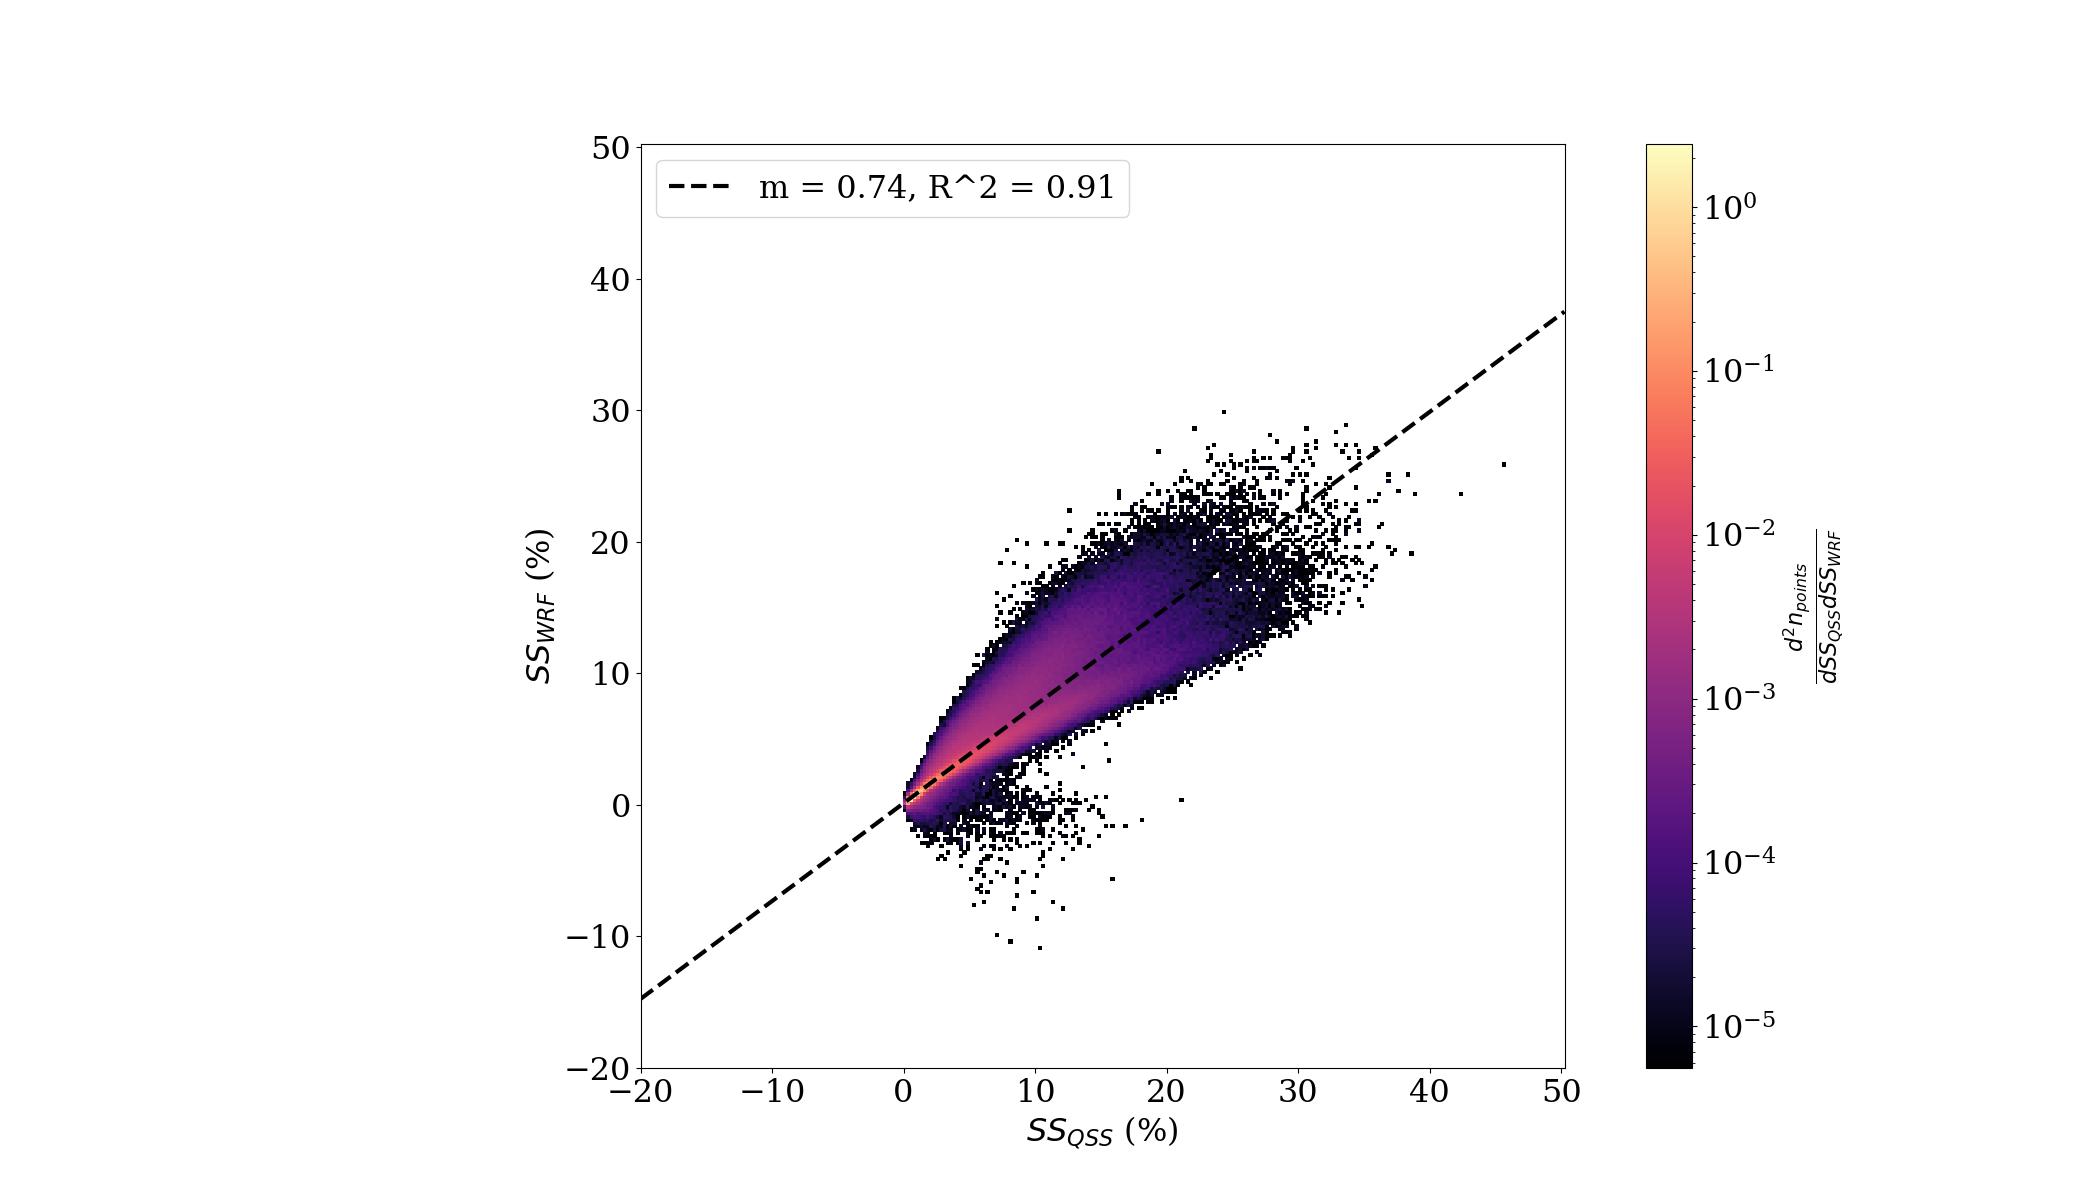
\includegraphics[width=\textwidth]{revmywrf/v1_FINAL_heatmap_ss_qss_vs_ss_wrf_Unpolluted_figure.png}
		\caption{Unpolluted case.}
		\label{wrfvsqssunpoll}
	\end{subfigure}
	\begin{subfigure}{0.7\textwidth}
		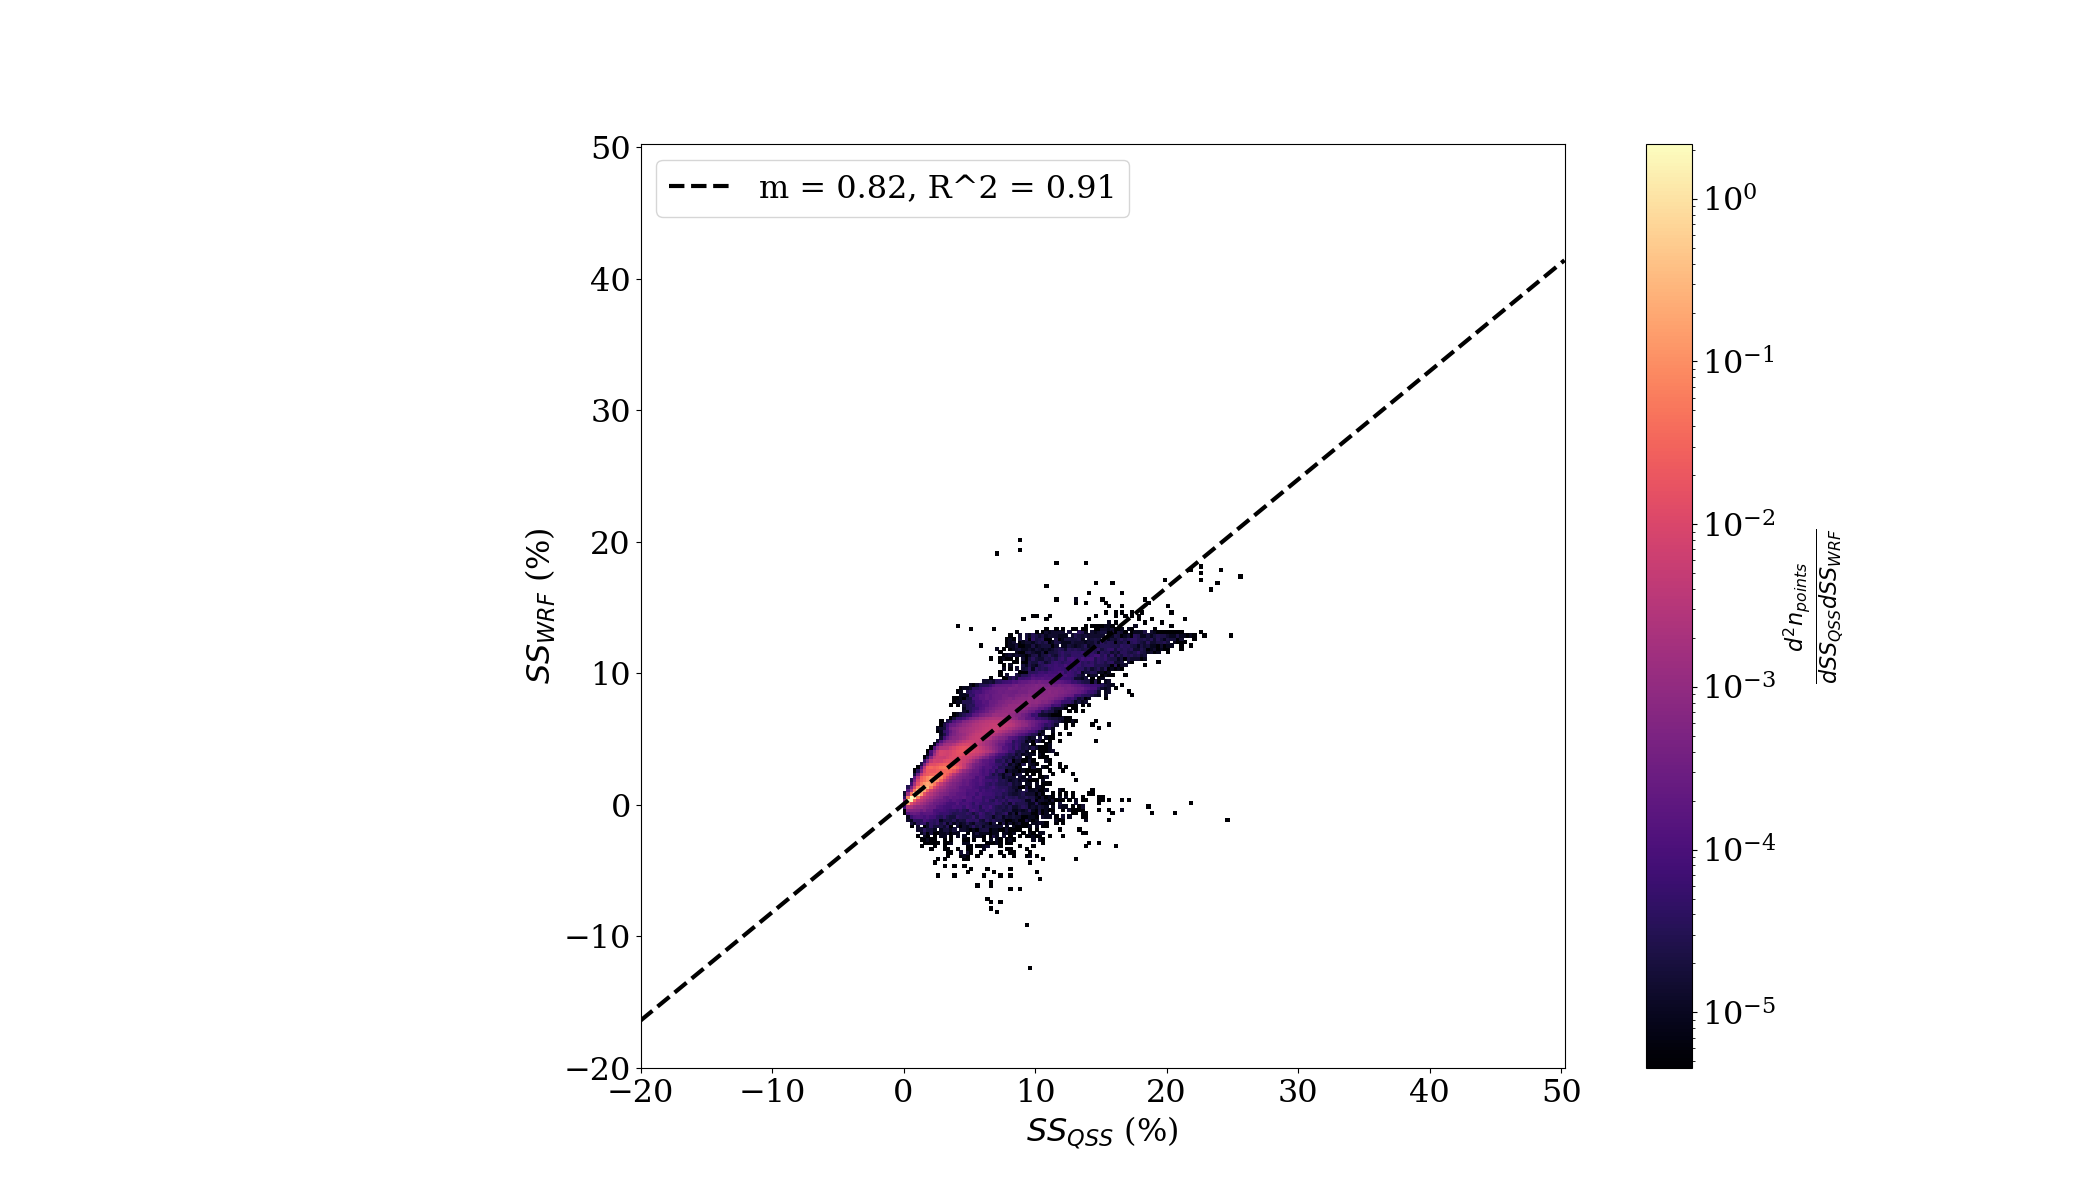
\includegraphics[width=\textwidth]{revmywrf/v1_FINAL_heatmap_ss_qss_vs_ss_wrf_Polluted_figure.png}
		\caption{Polluted case.}
		\label{wrfvsqsspoll}
	\end{subfigure}
	\caption{Actual ($SS_{WRF}$) vs predicted ($SS_{QSS}$) supersaturation. Color indicates density of data points; note the scale is logarithmic.}
	\label{wrfvsqss}
\end{figure}

Because we use slightly different filtering criteria than that employed in Fan et al to examine updrafts, we first verify that our selected cloudy updraft points yield similar SS profiles in the WRF simulation as those found in the latter work. In Figure \ref{wrfbipanel} we plot vertical SS profiles for all cloudy updraft points as well as the upper 10th percentile with respect to vertical wind velocity. We do indeed find the high SS values reported by Fan et al (maximum values of 13\% in both polluted and unpolluted cases from the upper 10th percentile dataset), confirming that our filtering criteria establish a fair basis for comparison here. Note however that, in the righthand panels of Figure \ref{wrfbipanel}, the vast majority of cloudy updraft points are found at altitudes with relatively low average SS.

\begin{figure}[ht]
	\centering
	\begin{subfigure}{0.7\textwidth}
		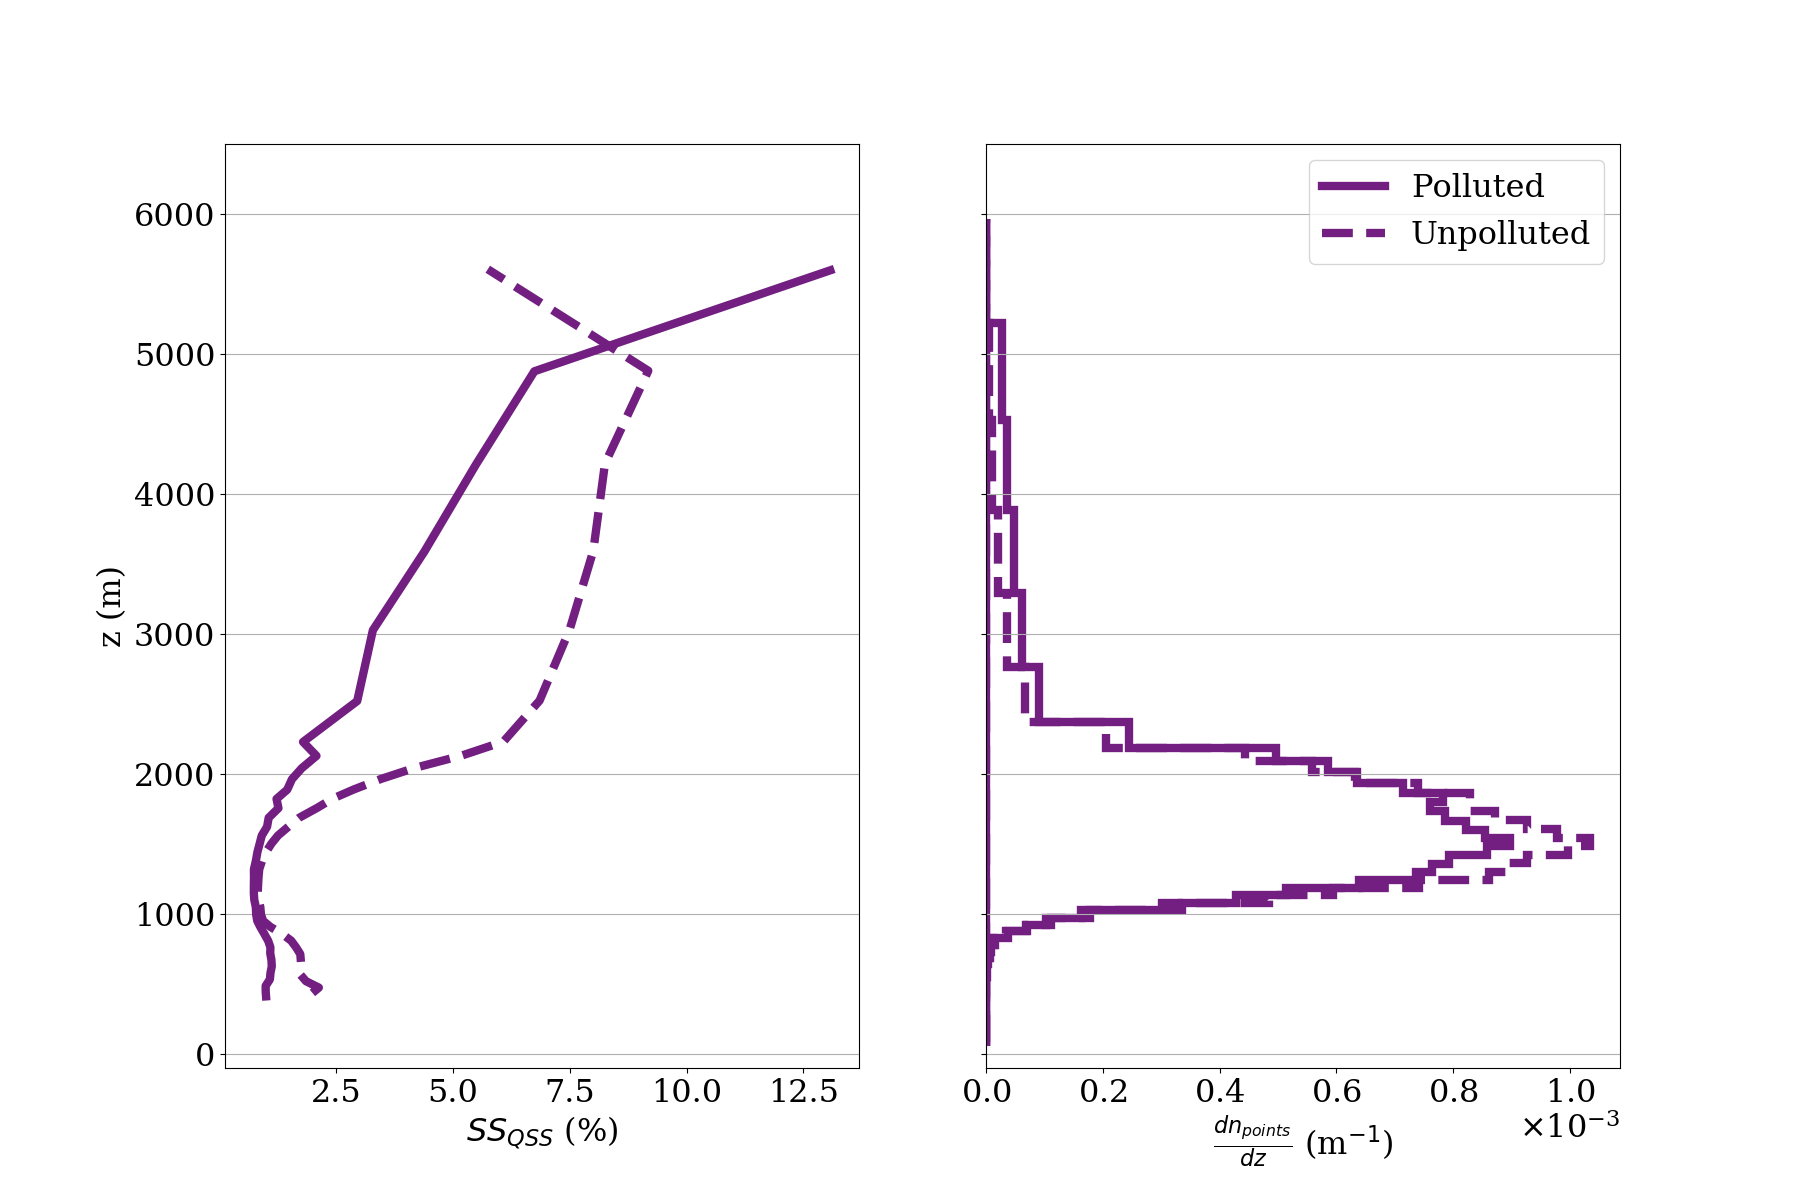
\includegraphics[width=\textwidth]{revmywrf/v4_FINAL_bipanel_ss_qss_vs_z_allpts_figure.png}
		\caption{}
		\label{wrfbipanelallpts}
	\end{subfigure}
	\begin{subfigure}{0.7\textwidth}
		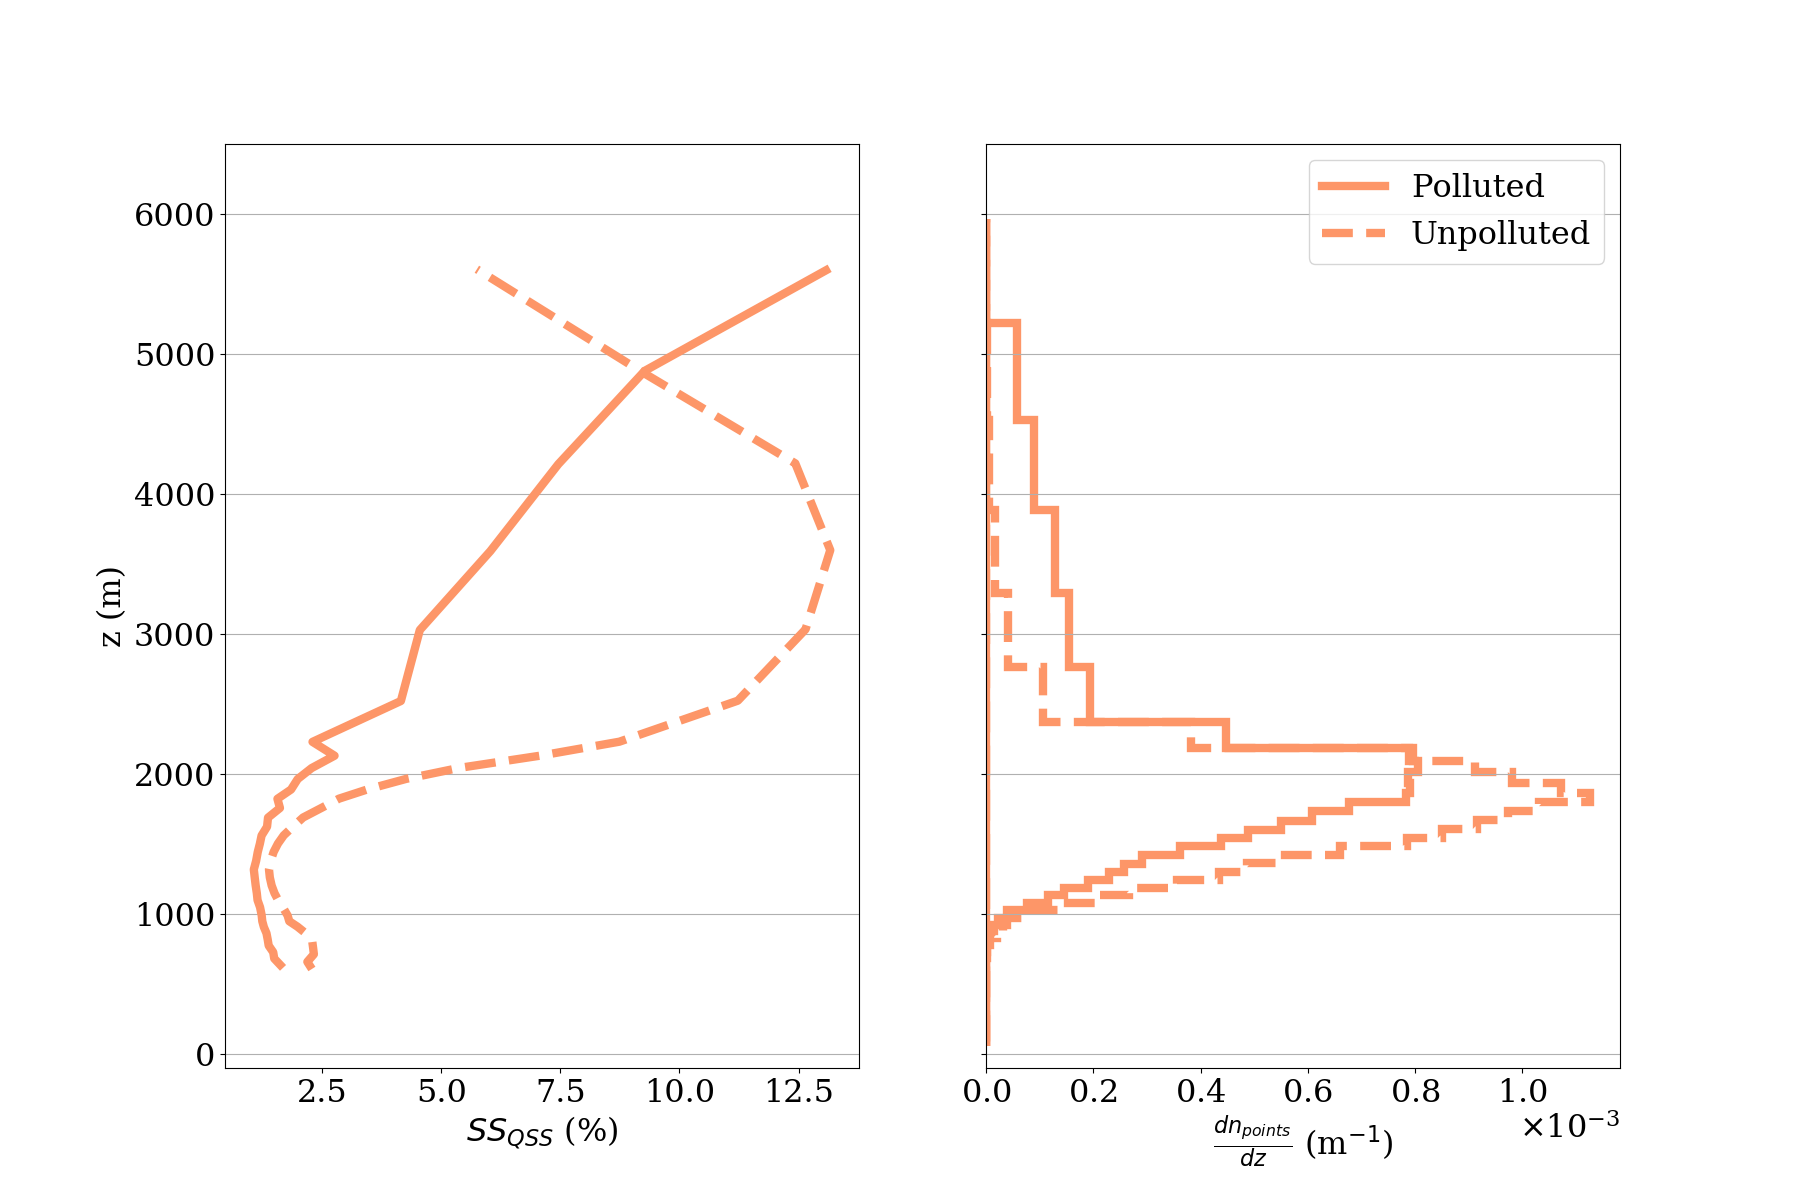
\includegraphics[width=\textwidth]{revmywrf/v4_FINAL_bipanel_ss_qss_vs_z_up10perc_figure.png}
		\caption{}
		\label{wrfbipanelup50perc}
	\end{subfigure}
	\caption{SS profiles (left) and number density of sampled points (right) for a) all cloudy updraft points; b) top 10\% of cloudy updraft points with respect to vertical wind velocity, in WRF simulation conducted by Fan et al. Each point in the vertical profile represents an average over all times and horizontal coordinates for a given vertical grid coordinate.}
	\label{wrfbipanel}
\end{figure}

\clearpage
\newpage

Here and henceforth, we compute the average over the vertical profile $SS(z)$ in the lefthand panels of Figure \ref{wrfbipanel} as:
\begin{equation}
\label{avgss}
\overline{SS} = \frac{\int dz SS(z)}{\int dz}
\end{equation}
For all cloudy updraft points in the WRF simulation (Figure \ref{wrfbipanel}(a)), $\overline{SS}$ equals 4.6\% and 5.7\% in the polluted and unpolluted cases, respectively; in the top 10\% of updrafts the average values are 5.8\% and 8.0\%. We do not show data for altitudes above the freezing line since the QSS approximation is invalid below the freezing temperature. However, let us take these average values as an approximation for the relative humidity difference between a hypothetical parcel and its environment over the scale height of the troposphere. Using our back-of-the-envelope derivation above, we calculate enhancements in CAPE relative to a temperature profile set by totally unsaturated storms of about 100 J/kg (top 10\% of updrafts), which (assuming no diffusive, frictional, or radiative losses) give an upper bound on increase in vertical wind velocity of $\approx$ 14 m/s.

We now seek to determine whether such high values actually occur in nature. First we look at data from the High-Altitude LOng-range research aircraft (HALO) (part of the ACRIDICON-CHUVA mission in Manaus, Brazil) [ \klcomm{how to cite?} ]. Figure \ref{halobipanel} shows the analogue of Figure \ref{wrfbipanel} using data from all HALO flight dates combined (see Methods/SI). Using the given vertical profiles we obtain $\overline{SS}$ of 0.26\% and 0.32\% for all cloudy updraft points and the upper 10\% of updrafts, respectively (note however that the average for the latter set is taken over a smaller vertical interval). Using the same methodology as above, this translates to an upper bound on increases in vertical velocity of roughly 3 m/s. 

\clearpage
\newpage

%\begin{figure}[ht]
%    \centering
%    \includegraphics[width=9cm]{atto/atto_psd_figure.png}
%    \caption{[DON'T HAVE DATA YET] Aerosol particle size distribution for a representative date; ground-based measurement coinciding with ACRIDICON-CHUVA flight dates, compared to initial distribution in boundary layer for WRF simulation. From ATTO site, upwind of Manaus metropolitan area.}
%    \label{attoasd}
%\end{figure}

%\begin{figure}[ht]
%    \centering
%    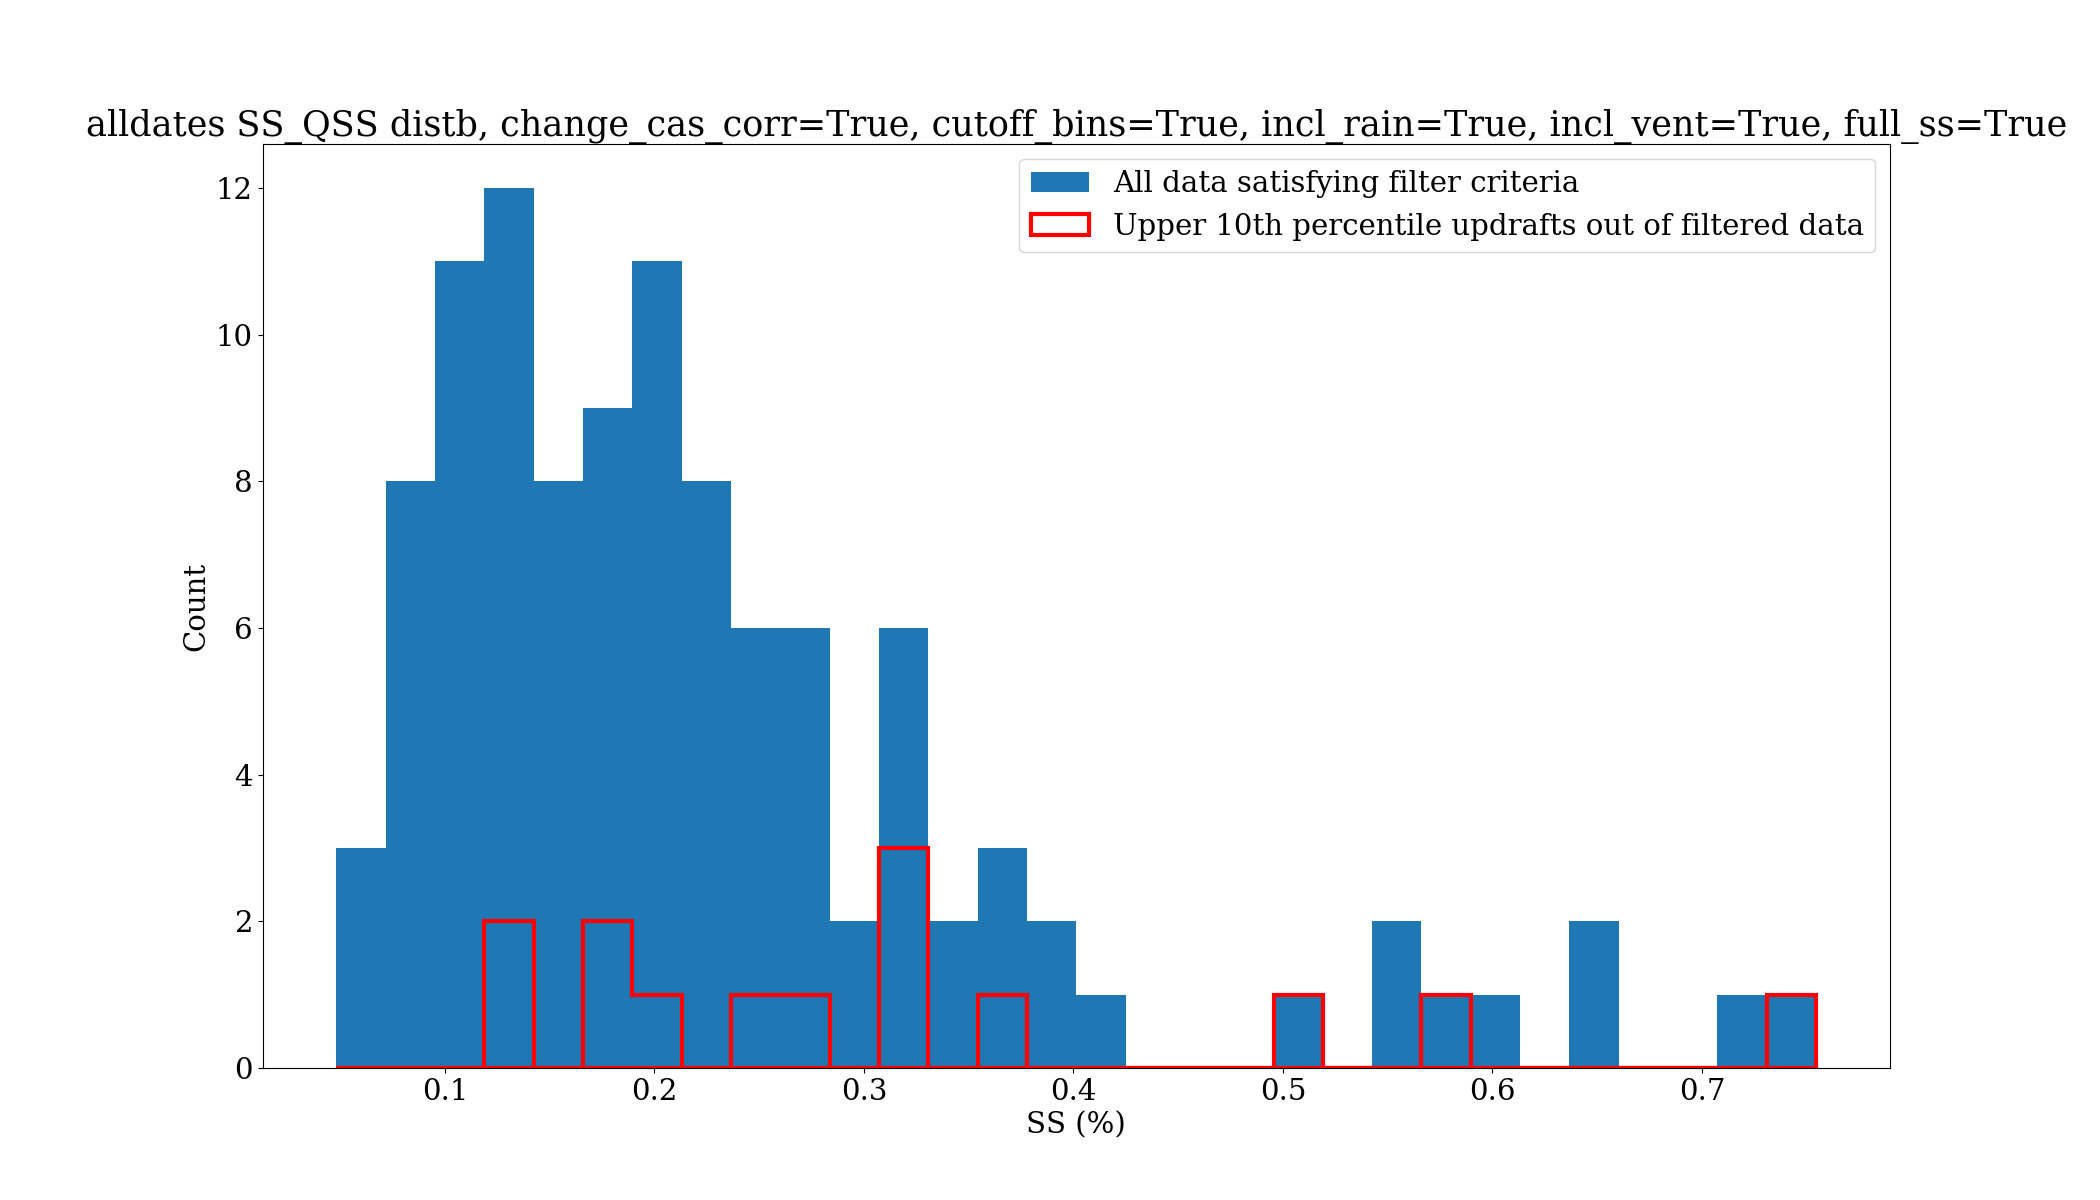
\includegraphics[width=9cm]{revhalo/v24_with_up10perc_ss_qss_hist_cas_alldates_figure.png}
%    \caption{Predicted ($SS_{QSS}$) supersaturation distribution from HALO field campaign (all flight dates). Using filtering criteria outlined in the text. Overlying histogram in red is the distribution for points lying in the upper tenth percentile of updrafts (as measured by vertical wind velocity), after Fan 2018.}
%    \label{haloqsshist}
%\end{figure}

\begin{figure}[ht]
    \centering
    \includegraphics[width=9cm]{revhalo/v1_FINAL_combined_bipanel_ss_qss_vs_z_figure.png}
    \caption{SS profiles (left) and number density of sampled points (right) from HALO flight campaign (all dates combined). Each point in the vertical profile represents an average over all times and horizontal coordinates for a given vertical interval (equally-spaced). SS profile is plotted with markers so as not to obscure intervals with missing data.}
    \label{halobipanel}
\end{figure}

Finally, we examine a second experimental dataset from the first phase of the Cloud Aerosol Interaction and Precipitation Enhancement Experiment (CAIPEEX) in India (taken in June [around Hyderabad] and August [around Bareilly] 2009) \cite{Kulkarni2012}. Although no UAP$_{<50}$ concentration measurements are available during this phase of the experiment, measurements of aerosols with diameters in the range of 0.1-3 $\mu$m showed total aerosol concentrations ranging from 700/ccm to 2500/ccm in the BL (see Figure 3(b) in \cite{Prabha2011} and Figure 4(a) in \cite{Kulkarni2012}). Reliable rain drop particle size distributions are unavailable from the flight dates in this analysis phase of the experiment, but we observe that exclusion of raindrops from the calculation of QSS SS leads to a systematic overestimation of the true SS (see Methods/SI). Therefore we take the SS profiles in Figure \ref{caipeexbipanel} as an upper bound; they yield $\overline{SS}$ of 0.52\% and 1.1\% for all cloudy updraft points and the upper 10\% of updrafts. This translates to maximal enhancements in vertical wind velocity of about 5 m/s for the upper 10th percentile.

%\begin{figure}[ht]
%    \centering
%    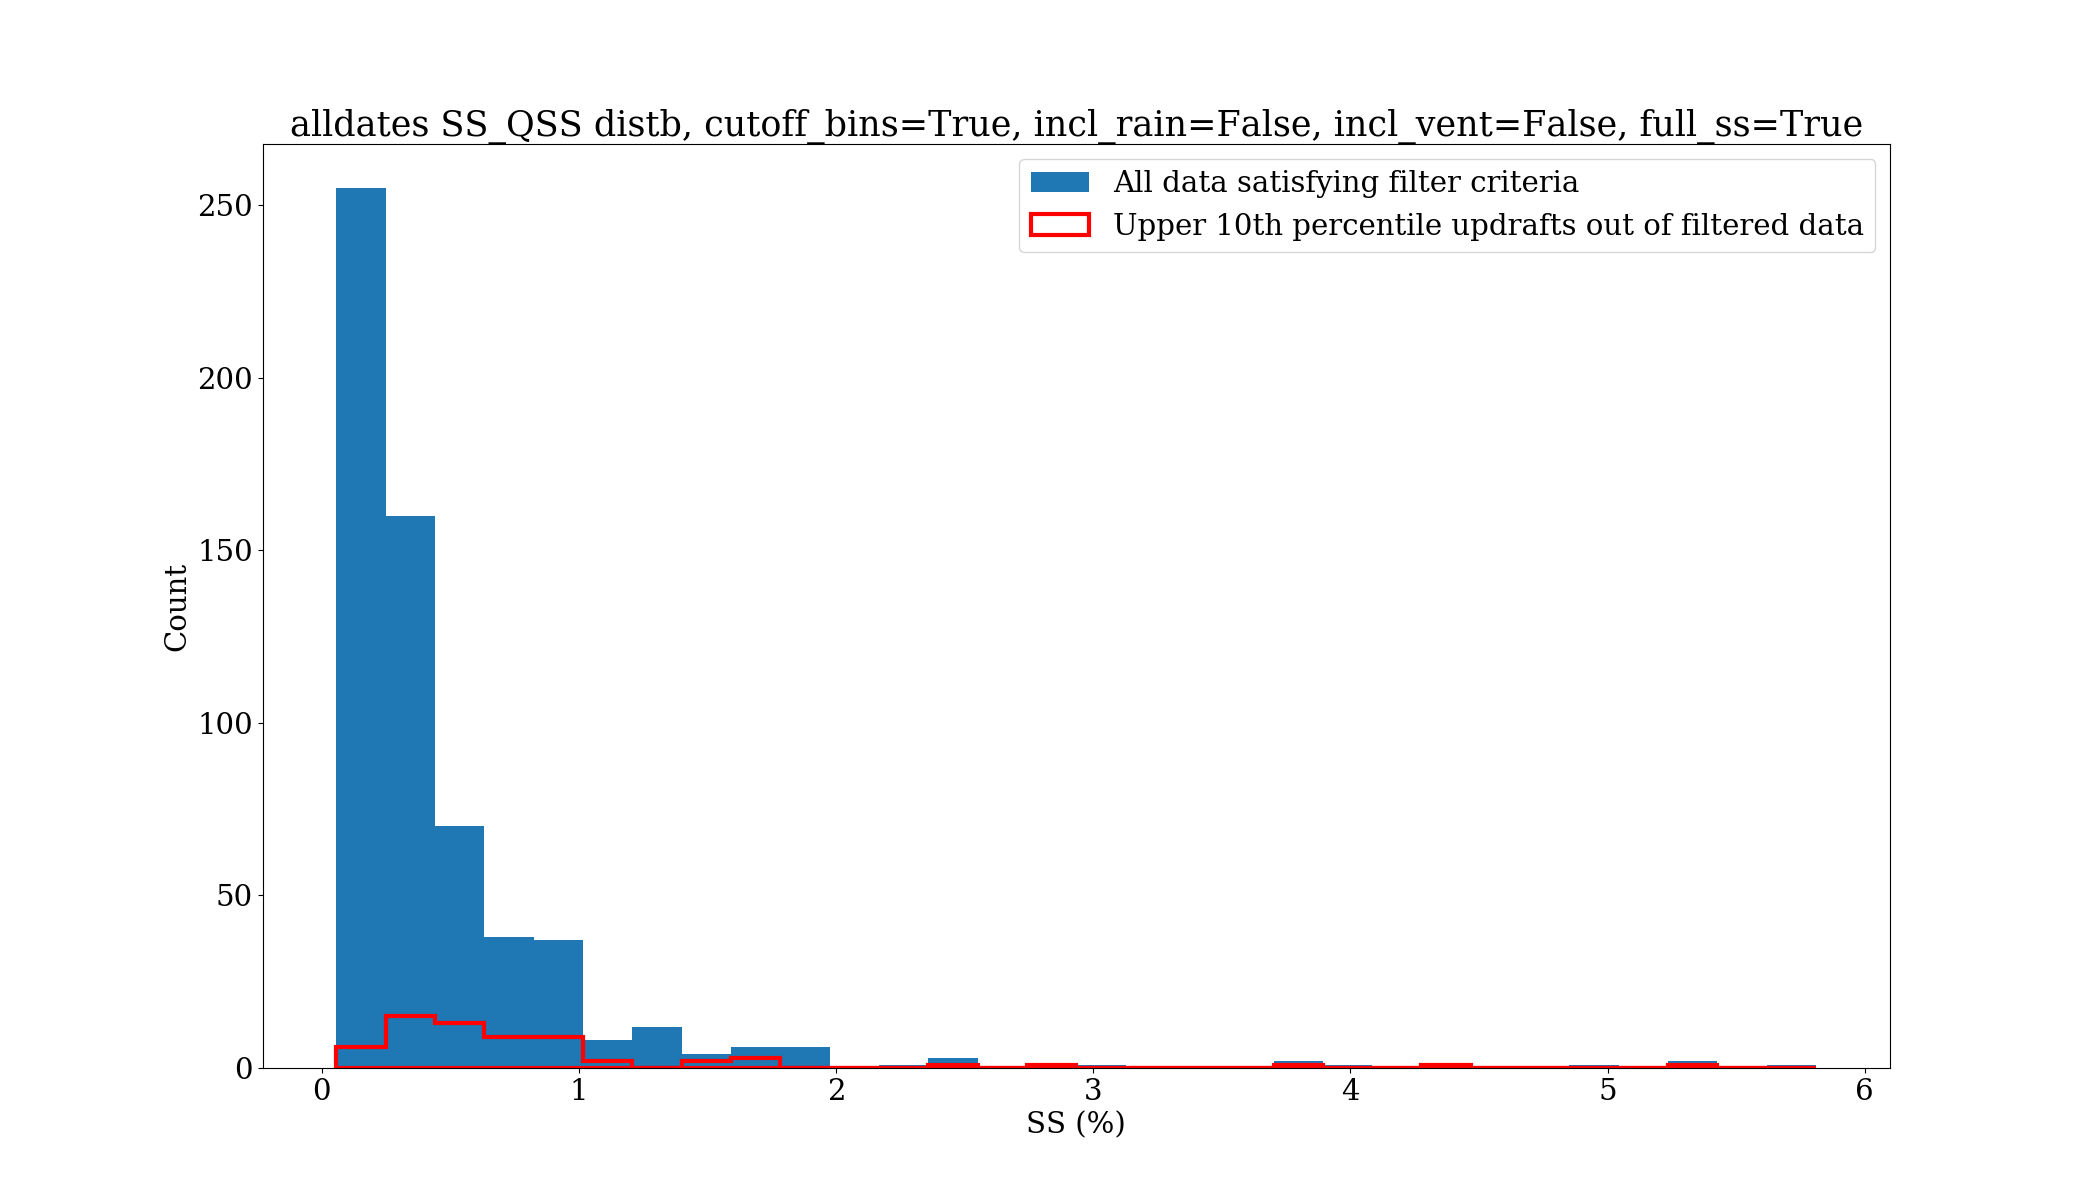
\includegraphics[width=9cm]{revcaipeex/v10_with_up10perc_ss_qss_hist_alldates_figure.png}
%    \caption{Predicted ($SS_{QSS}$) supersaturation distribution from CAIPEEX field campaign (all flight dates). Using filtering criteria outlined in the text, but not including rain drops or ventilation corrections due to lack of data. Overlying histogram in red is the distribution for points lying in the upper tenth percentile of updrafts (as measured by vertical wind velocity), after Fan 2018.}
%    \label{caipeexqsshist}
%\end{figure}

\begin{figure}[ht]
    \centering
    \includegraphics[width=9cm]{revcaipeex/v1_FINAL_combined_bipanel_ss_qss_vs_z_figure.png}
    \caption{SS profiles (left) and number density of sampled points (right) from CAIPEEX flight campaign (all dates combined). Each point in the vertical profile represents an average over all times and horizontal coordinates for a given vertical interval (equally-spaced). SS profile is plotted with markers so as not to obscure intervals with missing data. See text for comments on the dataset.}
    \label{caipeexbipanel}
\end{figure}

Conclusion: [ \klcomm{Trying my best to get the wording to be accurate and precise here but still not 100\% confident...} ] The WPIM as proposed by Fan et al requires the average temperature profile of the troposphere to be set by relatively clean (high-SS) convection, in order for more polluted (low-SS) convection to experience an enhancement in buoyancy. However, we find no evidence that the high SS values reported by Fan's model actually occur in nature, which weakens the possibility of measureable invigoration effects - in particular, we estimate an upper bound on vertical velocity enhancement of 3-5 m/s from the HALO and CAIPEEX flight campaigns, compared to roughly 14 m/s from Fan's control simulations in WRF. The relatively low aerosol concentrations used to initialize the simulations, in combination with possible irregularities in microphysical parameterizations, may be to blame for the anomalously high SS values in the WRF output.

One possible counterargument is that the aerosol concentrations in the BL during the dates of the HALO flights might have been significantly higher than those during the dates considered in Fan's paper, thus precluding the occurence of high SS values in the troposphere. In order to investigate this, we use the aerosol particle size distribution measured by the scanning mobility particle sizer (SMPS) in Manacapuru, located southwest of Manaus (PI: Chongai Kuang). This intrument measures particle concentrations in the diameter range 11.1-469.8nm. In Figure \ref{goamahist}, we show that, while we do indeed see higher total aerosol concentrations on average during the HALO flight date range (3500/ccm vs 2400/ccm), the UAP50 concentration is on average lower (1600/ccm vs 670/ccm). We note additionally that the aerosol concentrations used in the WRF simulations are much lower than those observed during the day the simulation takes place, which is not justified quantitatively in that study.
\begin{figure}[ht]
	\centering
	\begin{subfigure}{0.7\textwidth}
		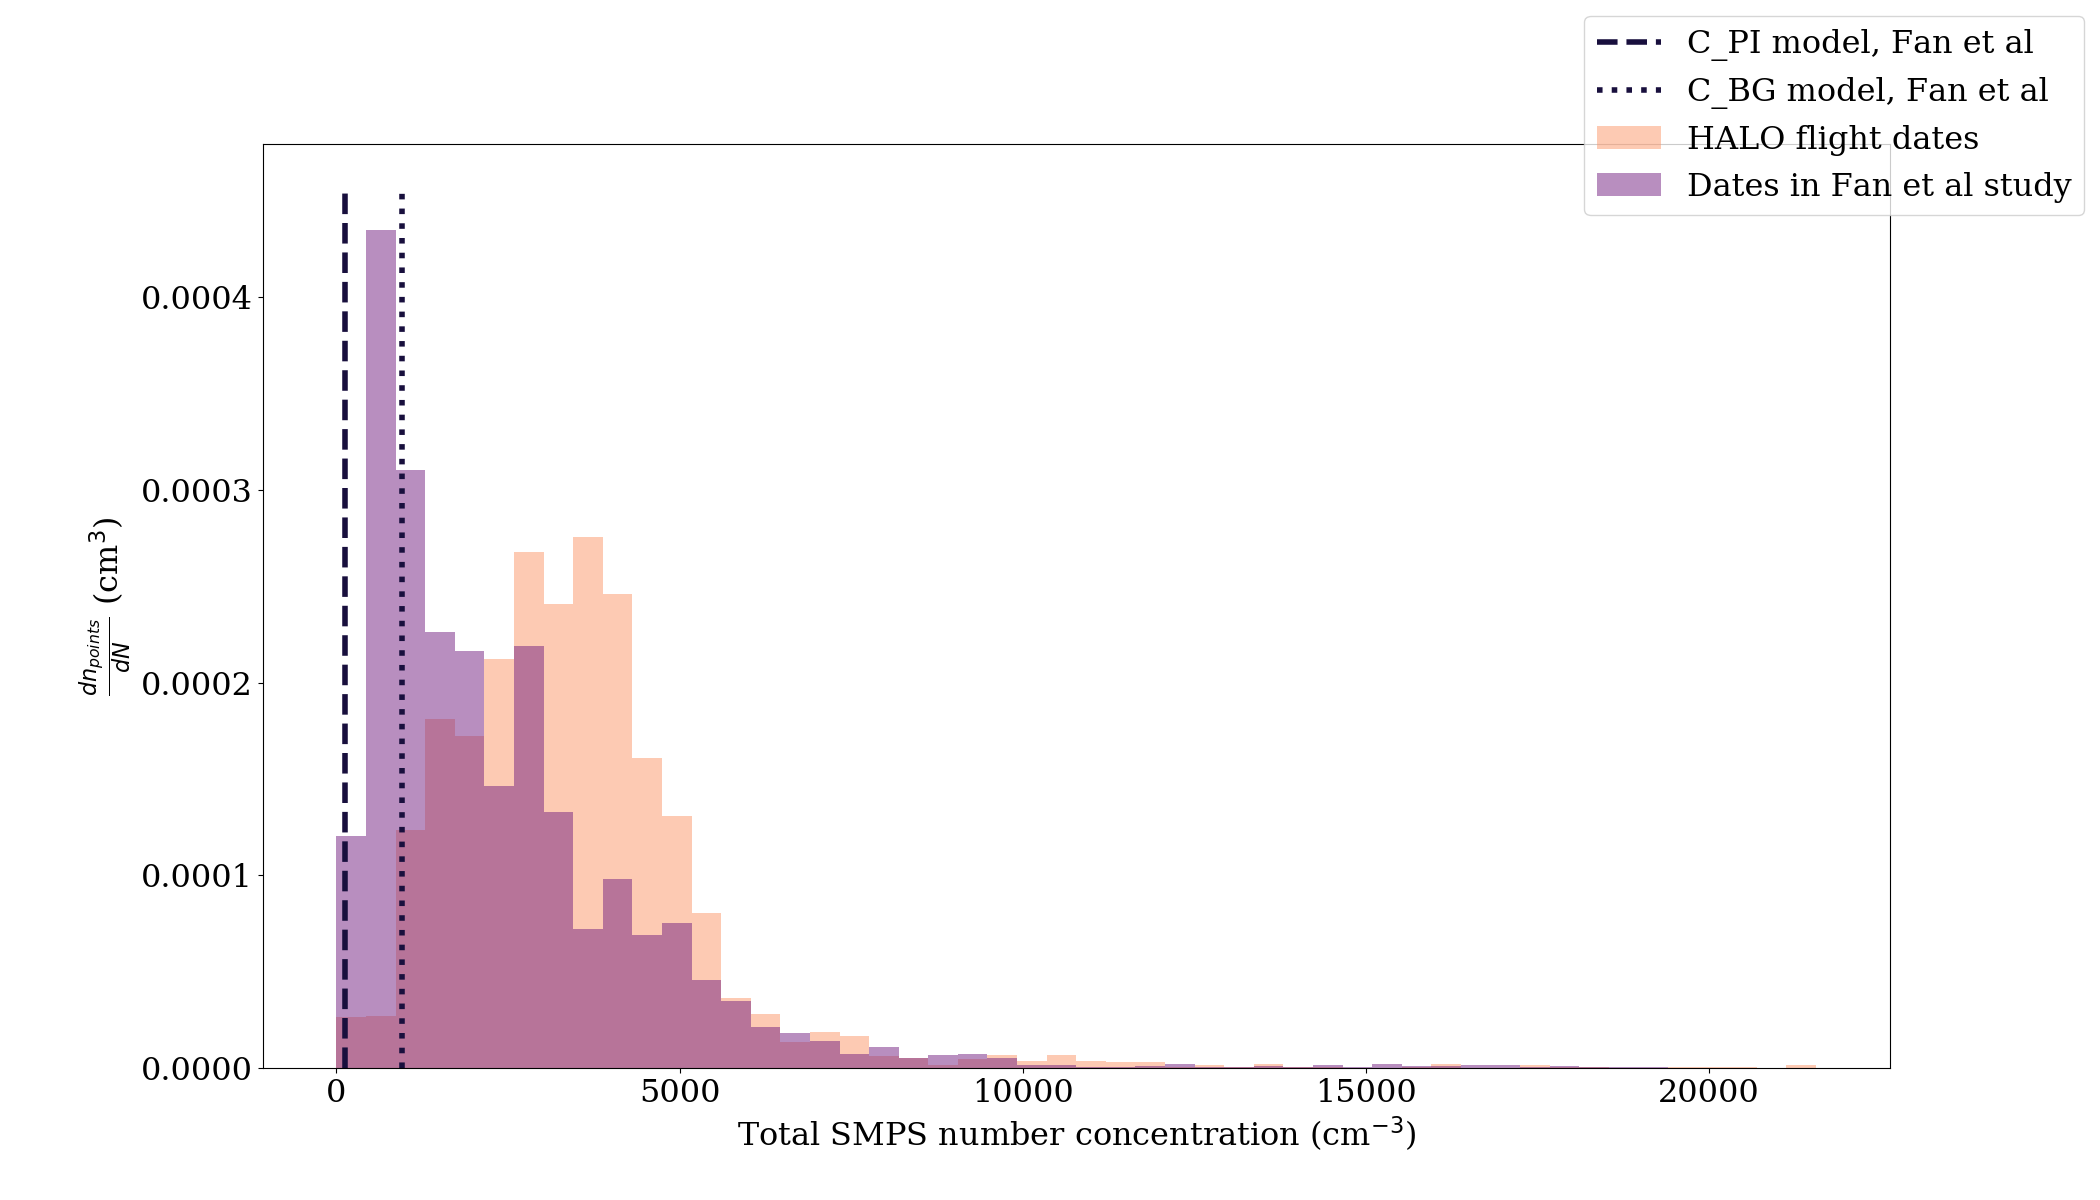
\includegraphics[width=\textwidth]{goama/v1_FINAL_tot_compare_nconc_hist_alldates_figure.png}
		\label{goamatothist}
		\caption{}
	\end{subfigure}
	\begin{subfigure}{0.7\textwidth}
		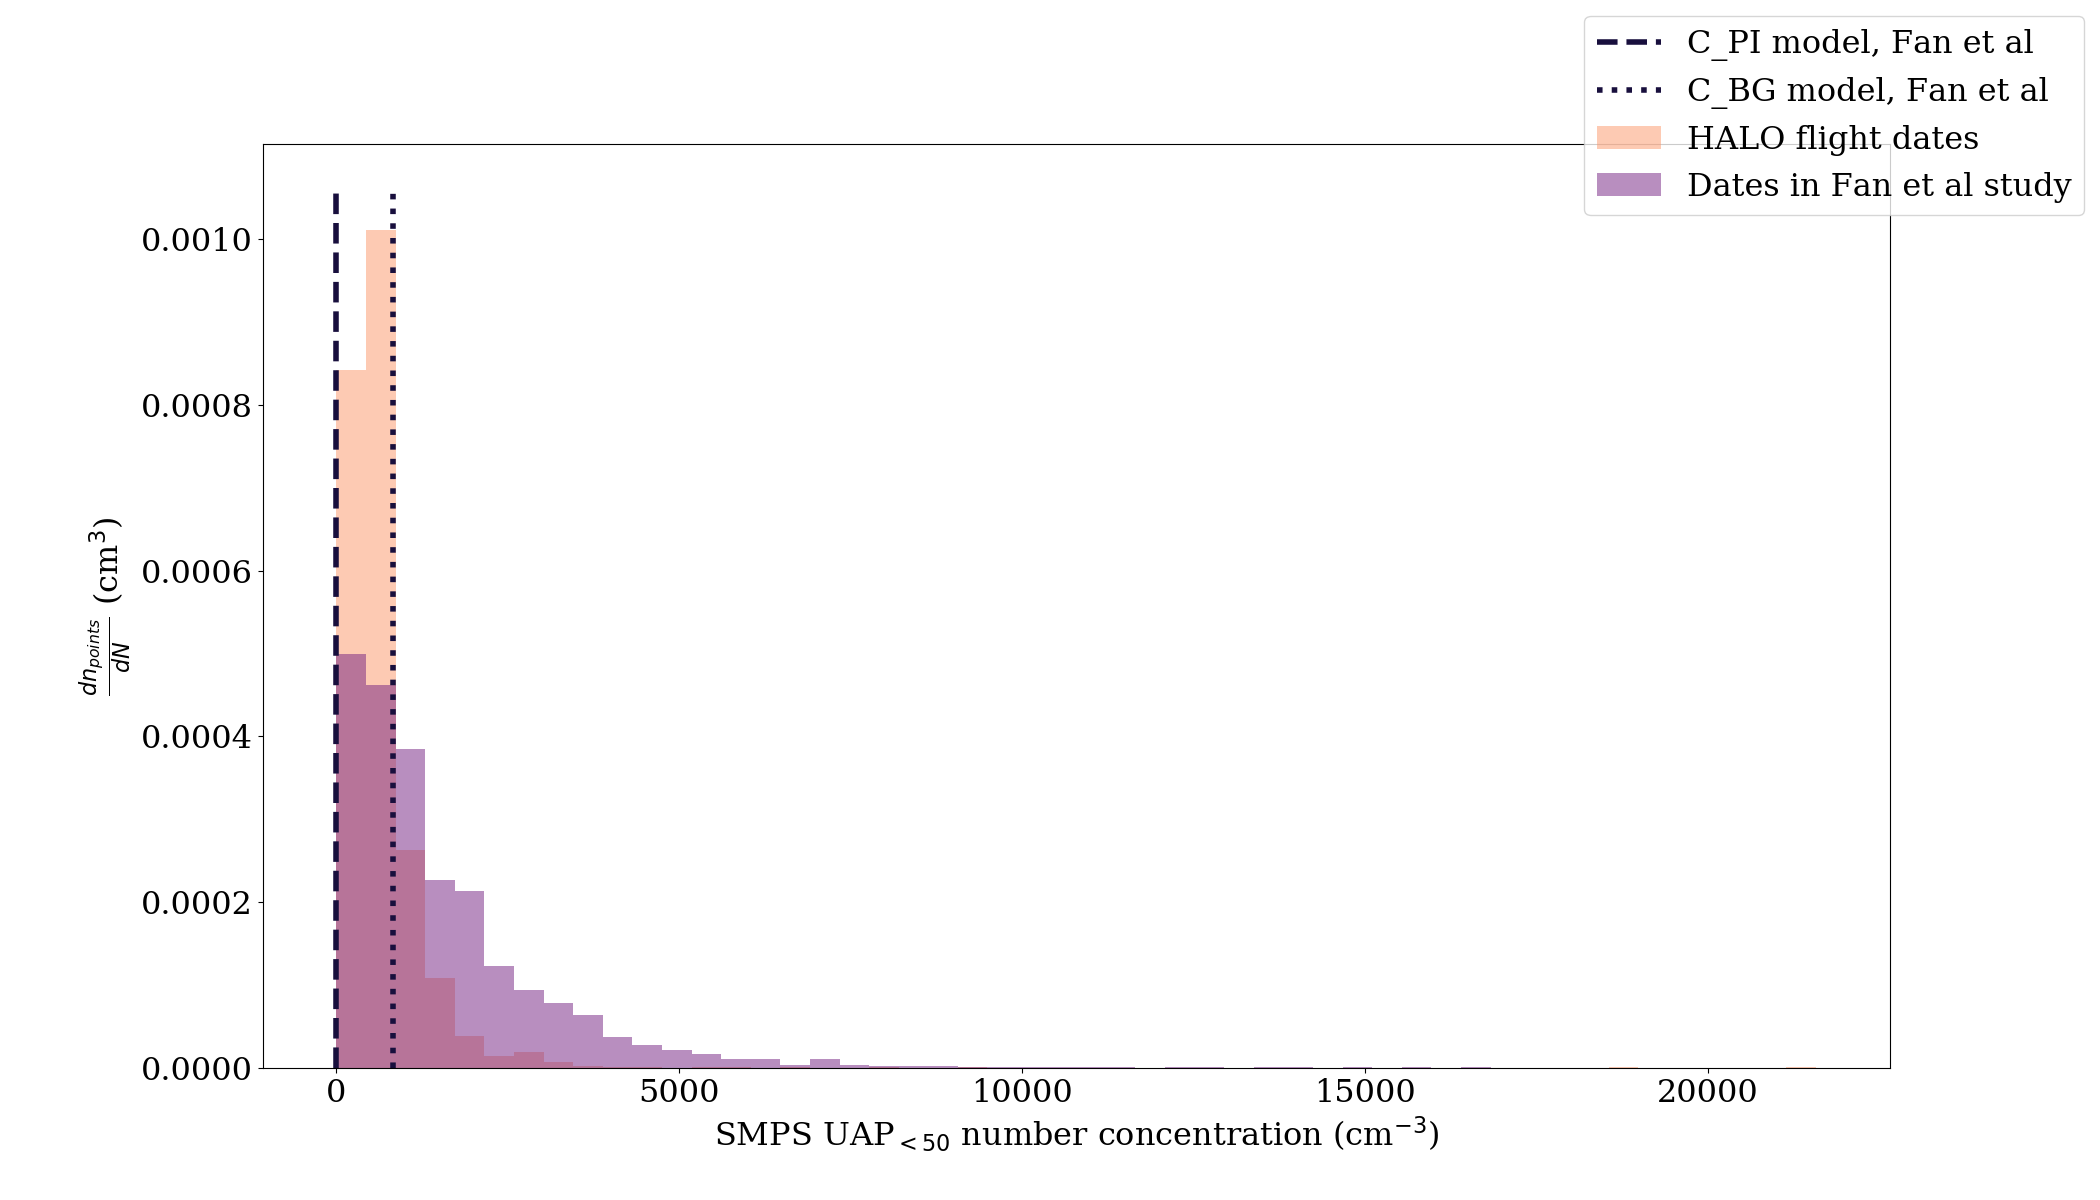
\includegraphics[width=\textwidth]{goama/v1_FINAL_uap50_compare_nconc_hist_alldates_figure.png}
		\label{goamauap50hist}
		\caption{}
	\end{subfigure}
	\caption{Distribution of aerosol concentration measurements by the ground-based SMPS at Manacapuru, Brazil; a) entire size range, b) only particles with diameter greater less than 50nm. HALO flight dates are the same as those represented in Figure \ref{halobipanel} (see Methods/SI for details). Dashed (dotted) lines show initial concentrations in the BL of the WRF simulation of polluted (unpolluted) conditions.}
	\label{goamahist}
\end{figure}

Another possible counterargument is that the flight campaigns simply didn't fly through strong enough updrafts. However the vertical velocity distributions from the campaigns are quite similar to that from the simulations. See Figure \ref{combinedwhist}. 

\begin{figure}[ht]
    \centering
    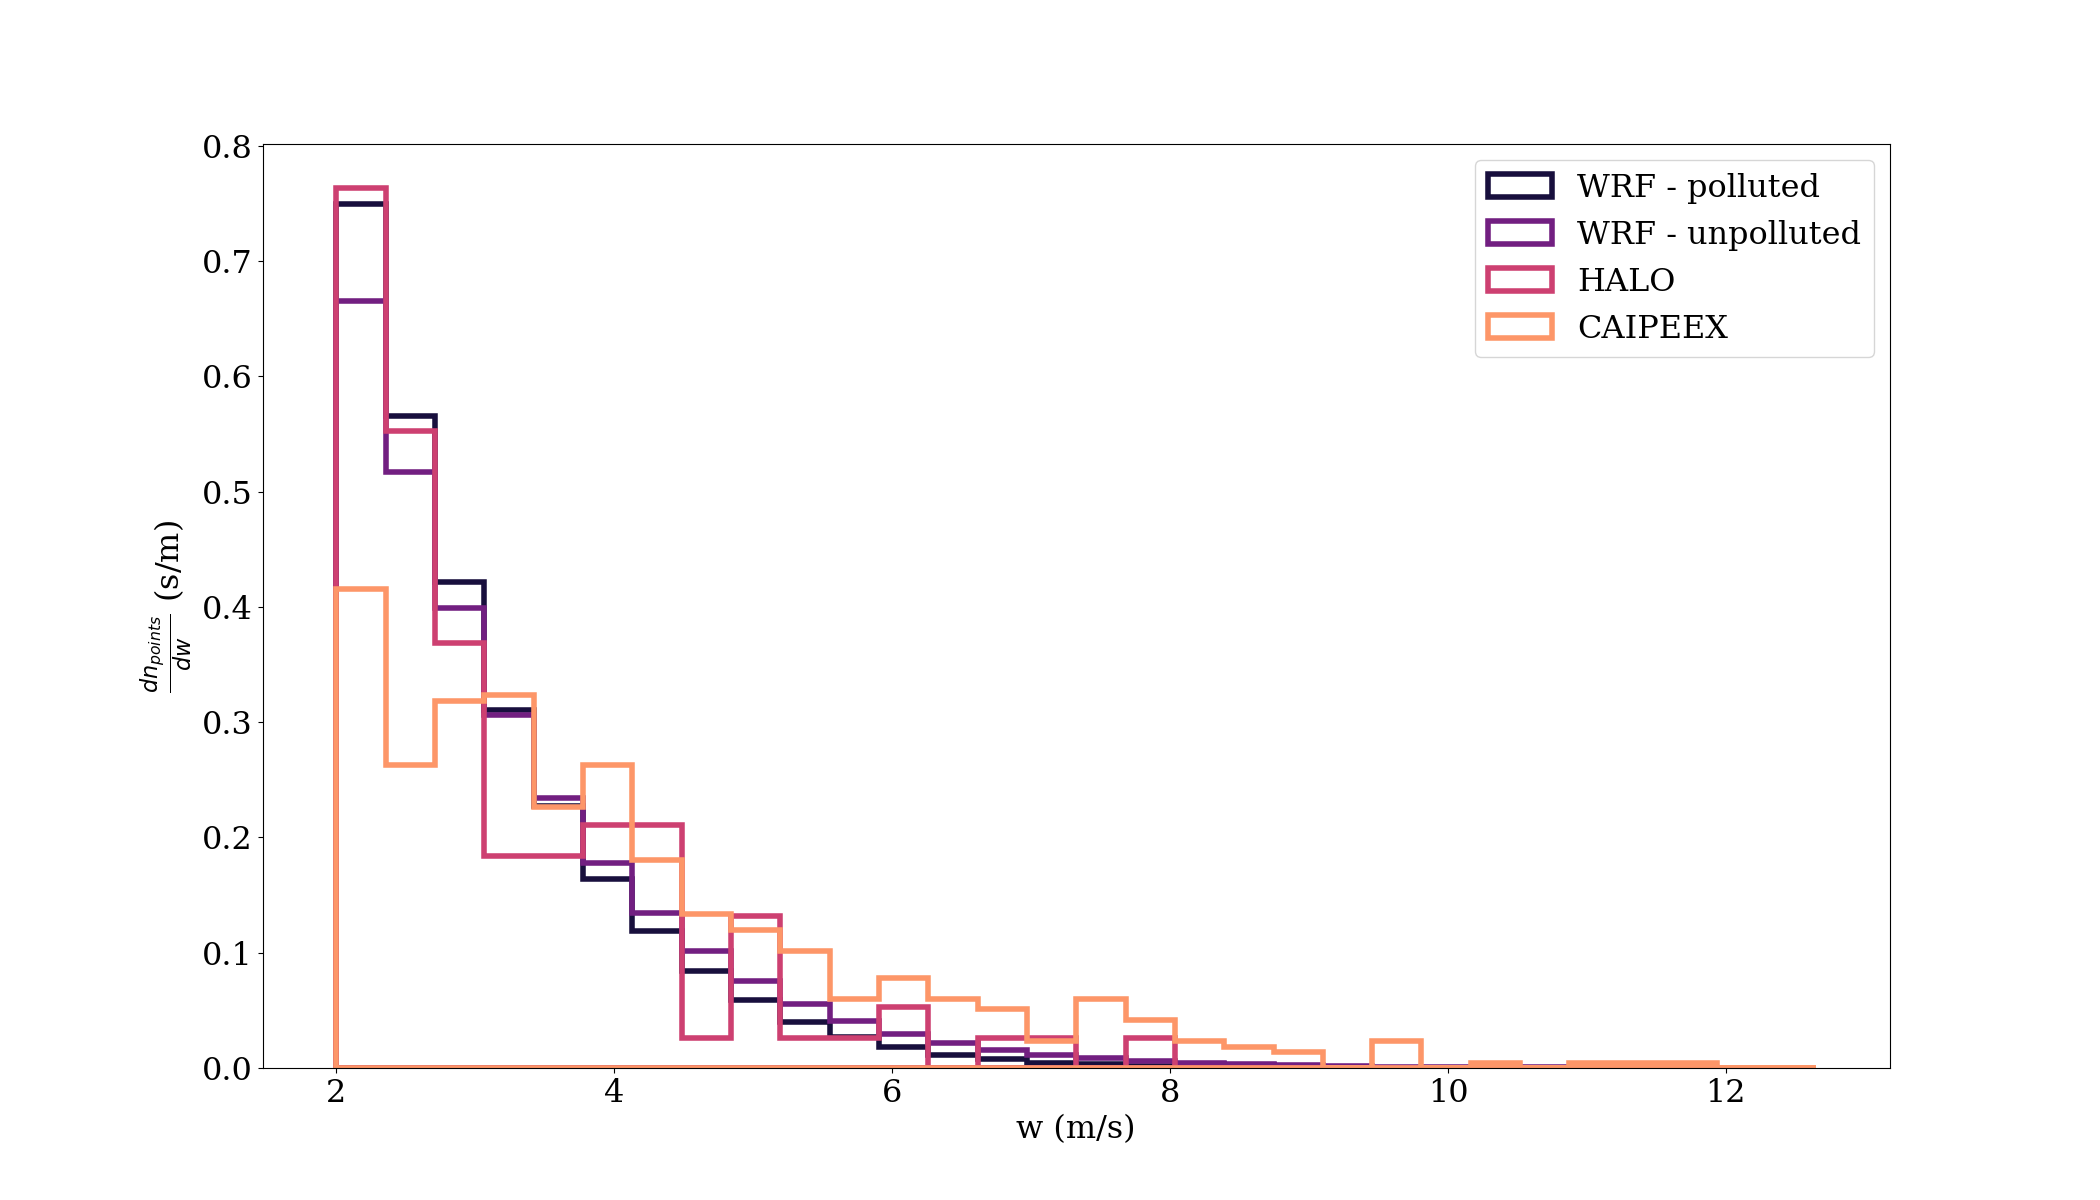
\includegraphics[width=12cm]{revmywrf/v1_FINAL_combined_w_hist_figure.png}
    \caption{Vertical wind velocity distribution from simulations and field campaigns. Using filtering criteria outlined in the text.}
    \label{combinedwhist}
\end{figure}

\clearpage
\newpage

\section{Methods/SI}

\subsection{WRF}

Model output for control simulations of polluted (``C\_BG") and unpolluted (``C\_PI") scenarios were provided by Fan et al; see that paper and accompanying SI for detailed explanations of model parameters and initializations.

In this paper, we use the following form of the QSS SS equation after \cite{Rogers1989} (with $SS_{QSS}$ given as a percentage):
\begin{equation}
\label{fullss}
SS_{QSS} = \frac{A(T) w}{4\pi B(\rho_a, T) \langle f(r)\cdot r\rangle n}*100,
\end{equation}
where:
\begin{align}
A(T) &= \frac{g}{R_a T}\Big(\frac{L_v R_a}{C_{ap} R_v T} - 1\Big)\big(F_d(T) + F_k(T)\big)\nonumber\\
F_d(T) &= \frac{\rho_w R_v T}{D e_s(T)}\nonumber\\
F_k(T) &= \Big(\frac{L_v}{R_v T} - 1\Big)\frac{L_v \rho_w}{K T}\nonumber\\
B(\rho_a, T) &= \rho_w\Big(\frac{R_v T}{e_s(T)} + \frac{L_v^2}{R_v C_{ap} \rho_a T^2}\Big)
\end{align}
Notation for constants and variables is given in Table \ref{vartable}. We use the following parameterization for $e_s$ \cite{Rogers1989}:
\begin{equation}
e_s(T) = 611.2e^{\frac{17.67T_c}{T_c + 243.5}},
\end{equation}
where $T_c$ is the temperature in degrees Celsius.

We note that this equation by also include finite size correction terms; however, using typical values for droplet salinity and condensation nucleus radius (the relevant parameters in this case), these terms are insignificant ($<$ 0.1\% correction to SS) for drops of radius greater than 3 $\mu$m \cite{Rogers1989}, and we therefore do not consider them in this paper.

A simpler form of Equation \ref{fullss} is often employed in the literature \cite{Grabowski2020, Rogers1989}, with:
\begin{align}
A(T) &= \frac{g}{R_a T}\Big(\frac{L_v R_a}{C_{ap} R_v T} - 1\Big)\nonumber\\
B(T) &= D
\end{align}
Figure \ref{wrfvsqssv2} shows that this form does not yield as good of agreement with the actual SS reported in WRF.

\begin{figure}[ht]
	\centering
	\begin{subfigure}{0.7\textwidth}
		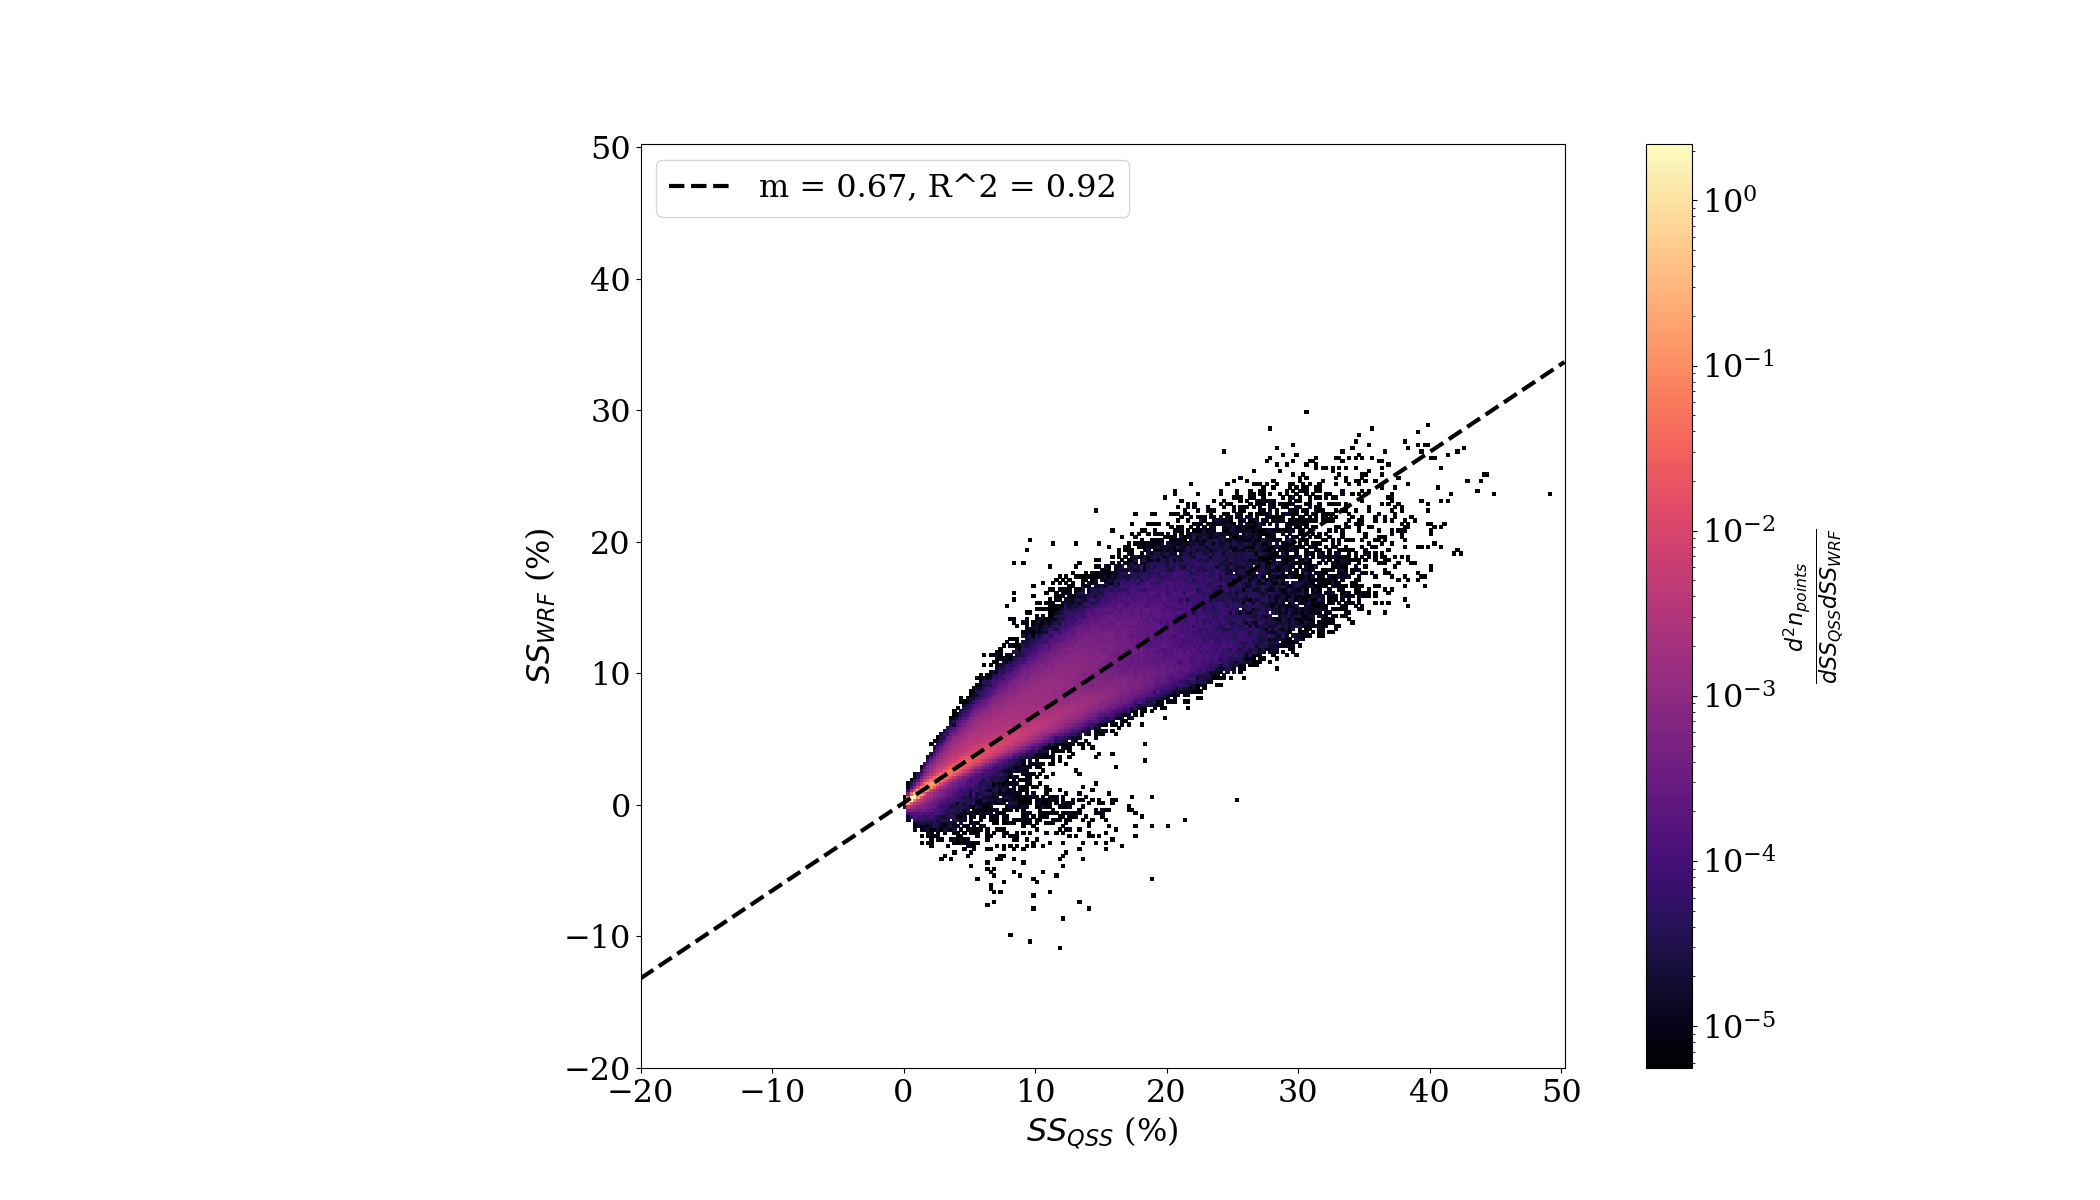
\includegraphics[width=\textwidth]{revmywrf/v2_FINAL_heatmap_ss_qss_vs_ss_wrf_Unpolluted_figure.png}
		\caption{Unpolluted case.}
		\label{wrfvsqssunpollv2}
	\end{subfigure}
	\begin{subfigure}{0.7\textwidth}
		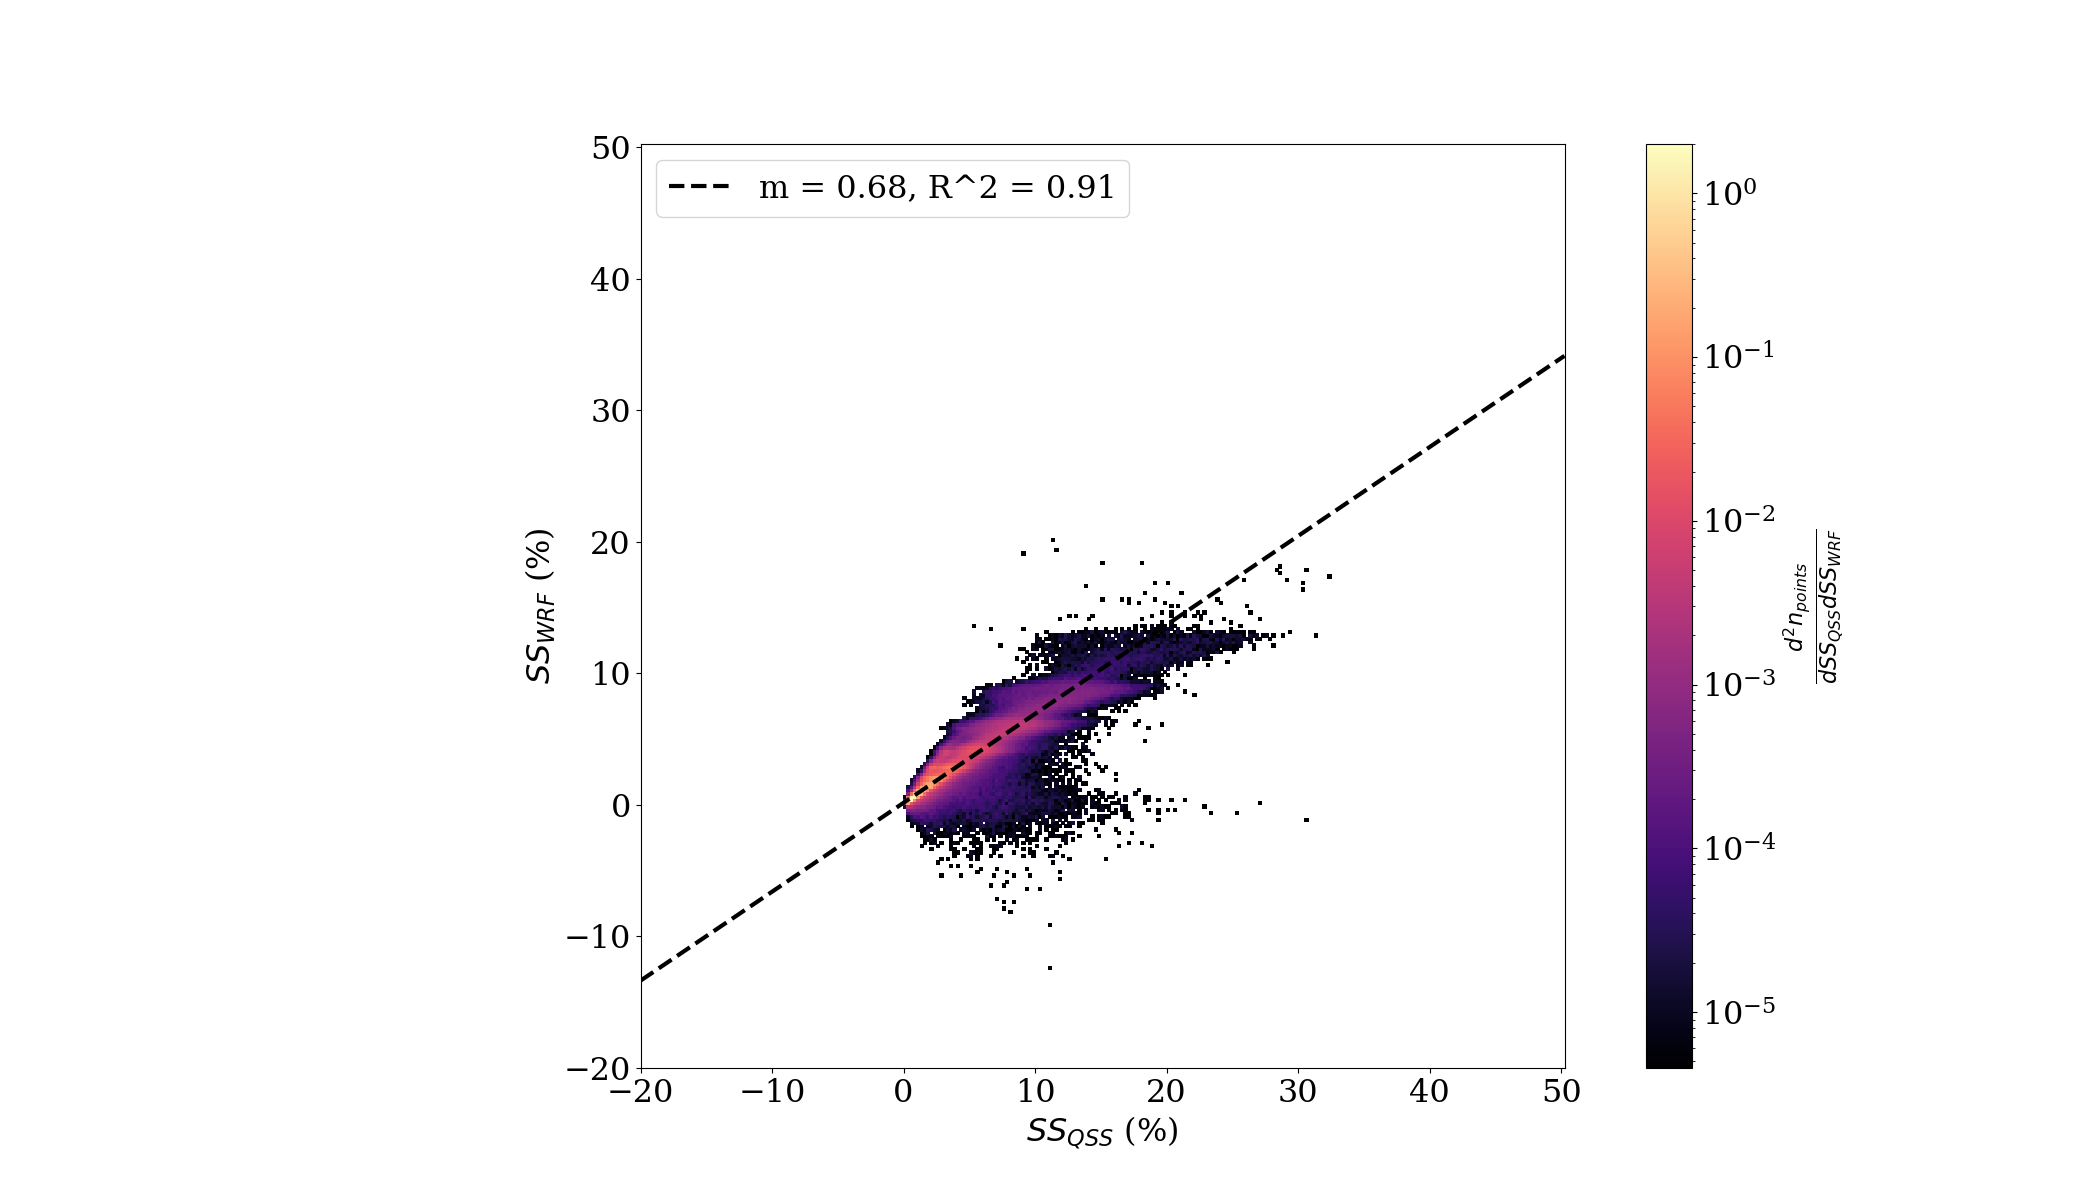
\includegraphics[width=\textwidth]{revmywrf/v2_FINAL_heatmap_ss_qss_vs_ss_wrf_Polluted_figure.png}
		\caption{Polluted case.}
		\label{wrfvsqsspollv2}
	\end{subfigure}
	\caption{Actual ($SS_{WRF}$) vs predicted ($SS_{QSS}$) supersaturation, using simplified form of Equation \ref{fullss}. Color indicates density of data points; note the scale is logarithmic.}
	\label{wrfvsqssv2}
\end{figure}

We use the expressions given in \cite{Pruppacher2010} and \cite{Rogers1989} for ventilation corrections [ \klcomm{They are kind of extensive...should I write out all formulae or just refer to the code in GitHub?} ]. Figures \ref{wrfvsqssv3} and \ref{wrfvsqssv5} show, respectively, the effects of neglecting these corrections (i.e. setting $f(r)=1$ for all $r$) for rain drops (defined here as liquid water drops with diameter greater than 50 $\mu$m), and omitting rain drops altogether from the calculations of mean radius and number concentration.

\begin{figure}[ht]
	\centering
	\begin{subfigure}{0.7\textwidth}
		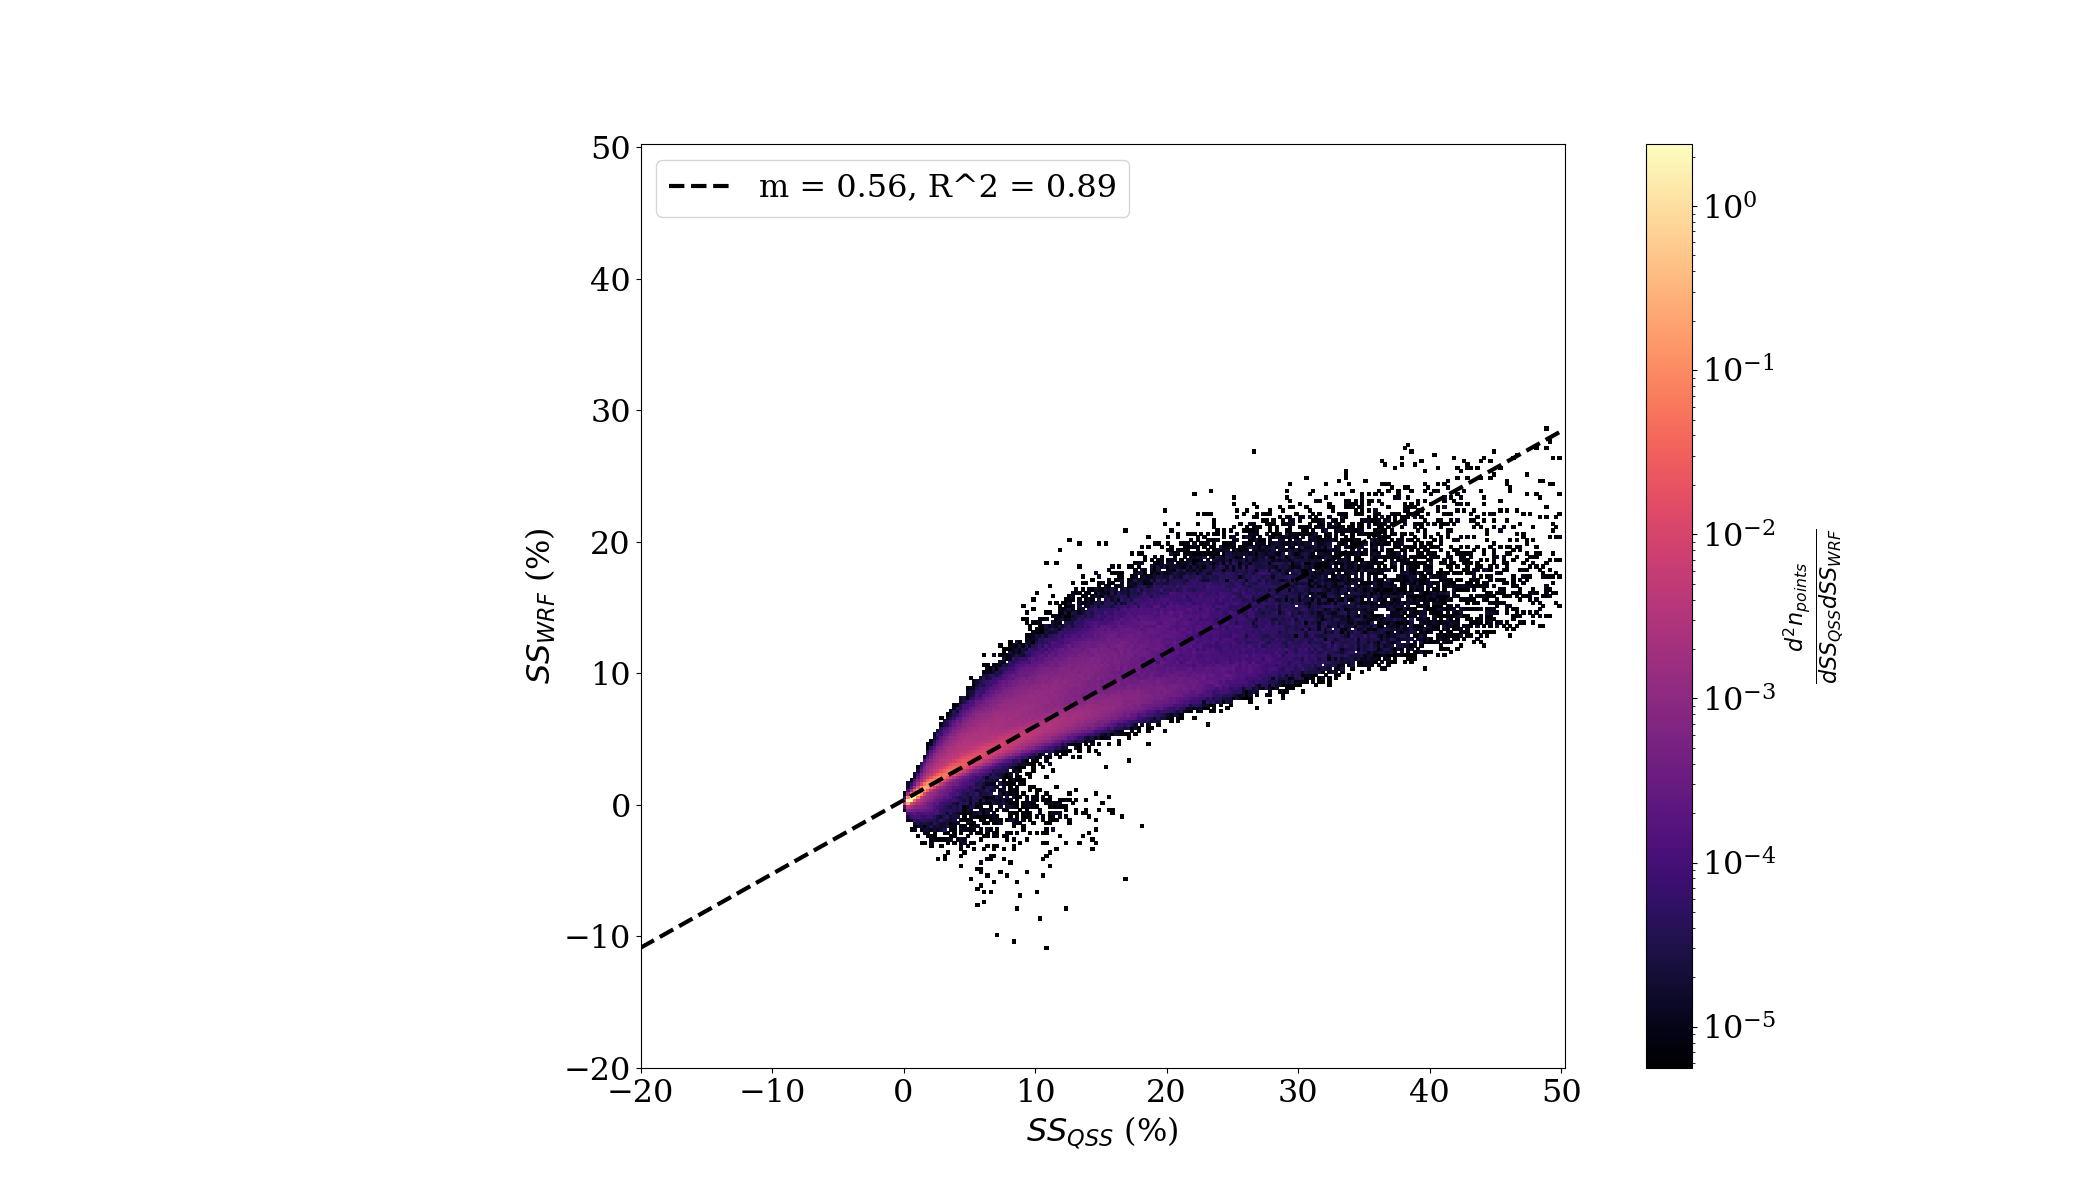
\includegraphics[width=\textwidth]{revmywrf/v3_FINAL_heatmap_ss_qss_vs_ss_wrf_Unpolluted_figure.png}
		\caption{Unpolluted case.}
		\label{wrfvsqssunpollv3}
	\end{subfigure}
	\begin{subfigure}{0.7\textwidth}
		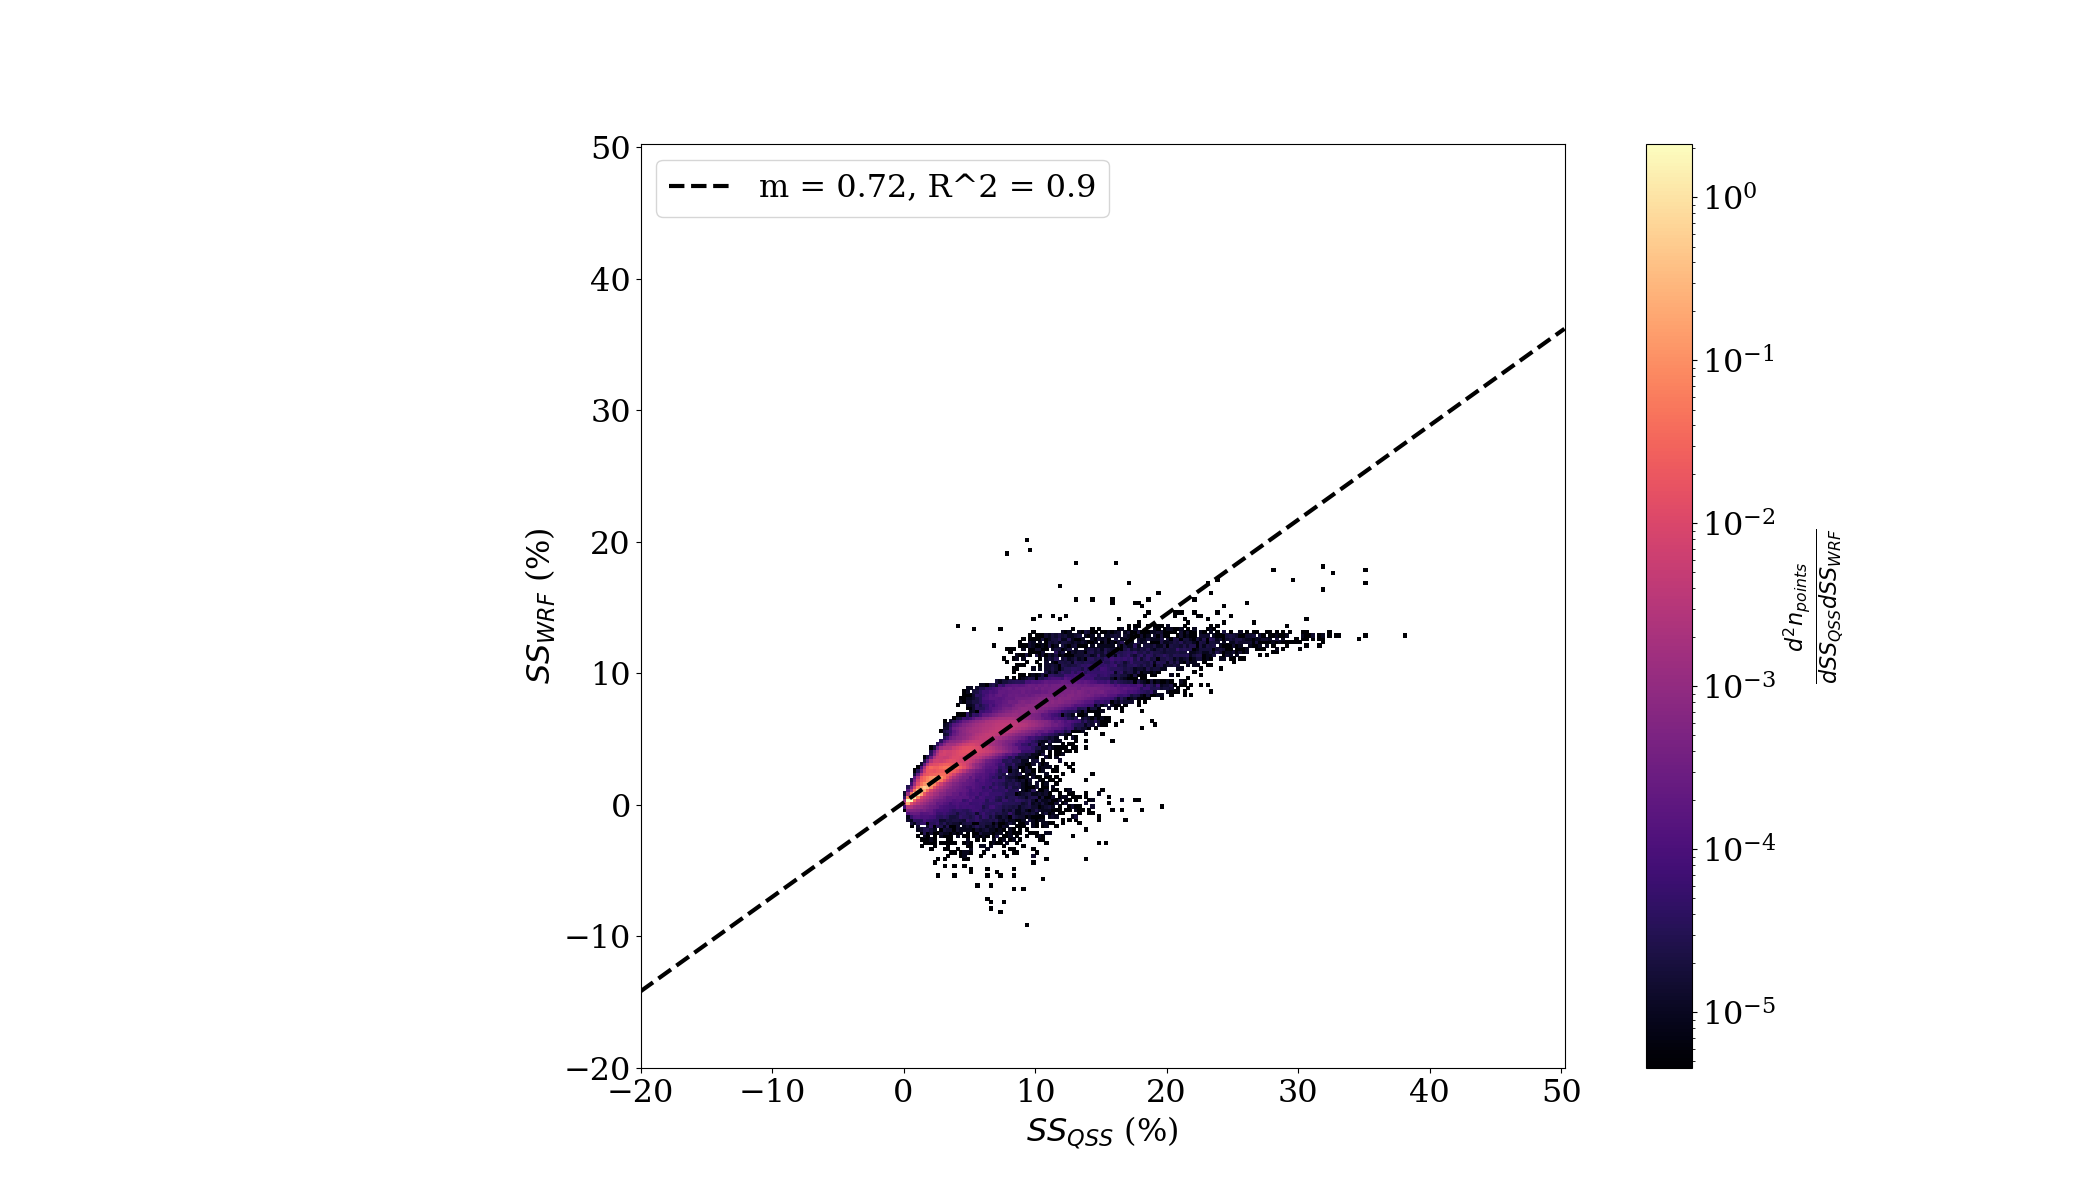
\includegraphics[width=\textwidth]{revmywrf/v3_FINAL_heatmap_ss_qss_vs_ss_wrf_Polluted_figure.png}
		\caption{Polluted case.}
		\label{wrfvsqsspollv3}
	\end{subfigure}
	\caption{Actual ($SS_{WRF}$) vs predicted ($SS_{QSS}$) supersaturation, without ventilation corrections. Color indicates density of data points; note the scale is logarithmic.}
	\label{wrfvsqssv3}
\end{figure}

\begin{figure}[ht]
	\centering
	\begin{subfigure}{0.7\textwidth}
		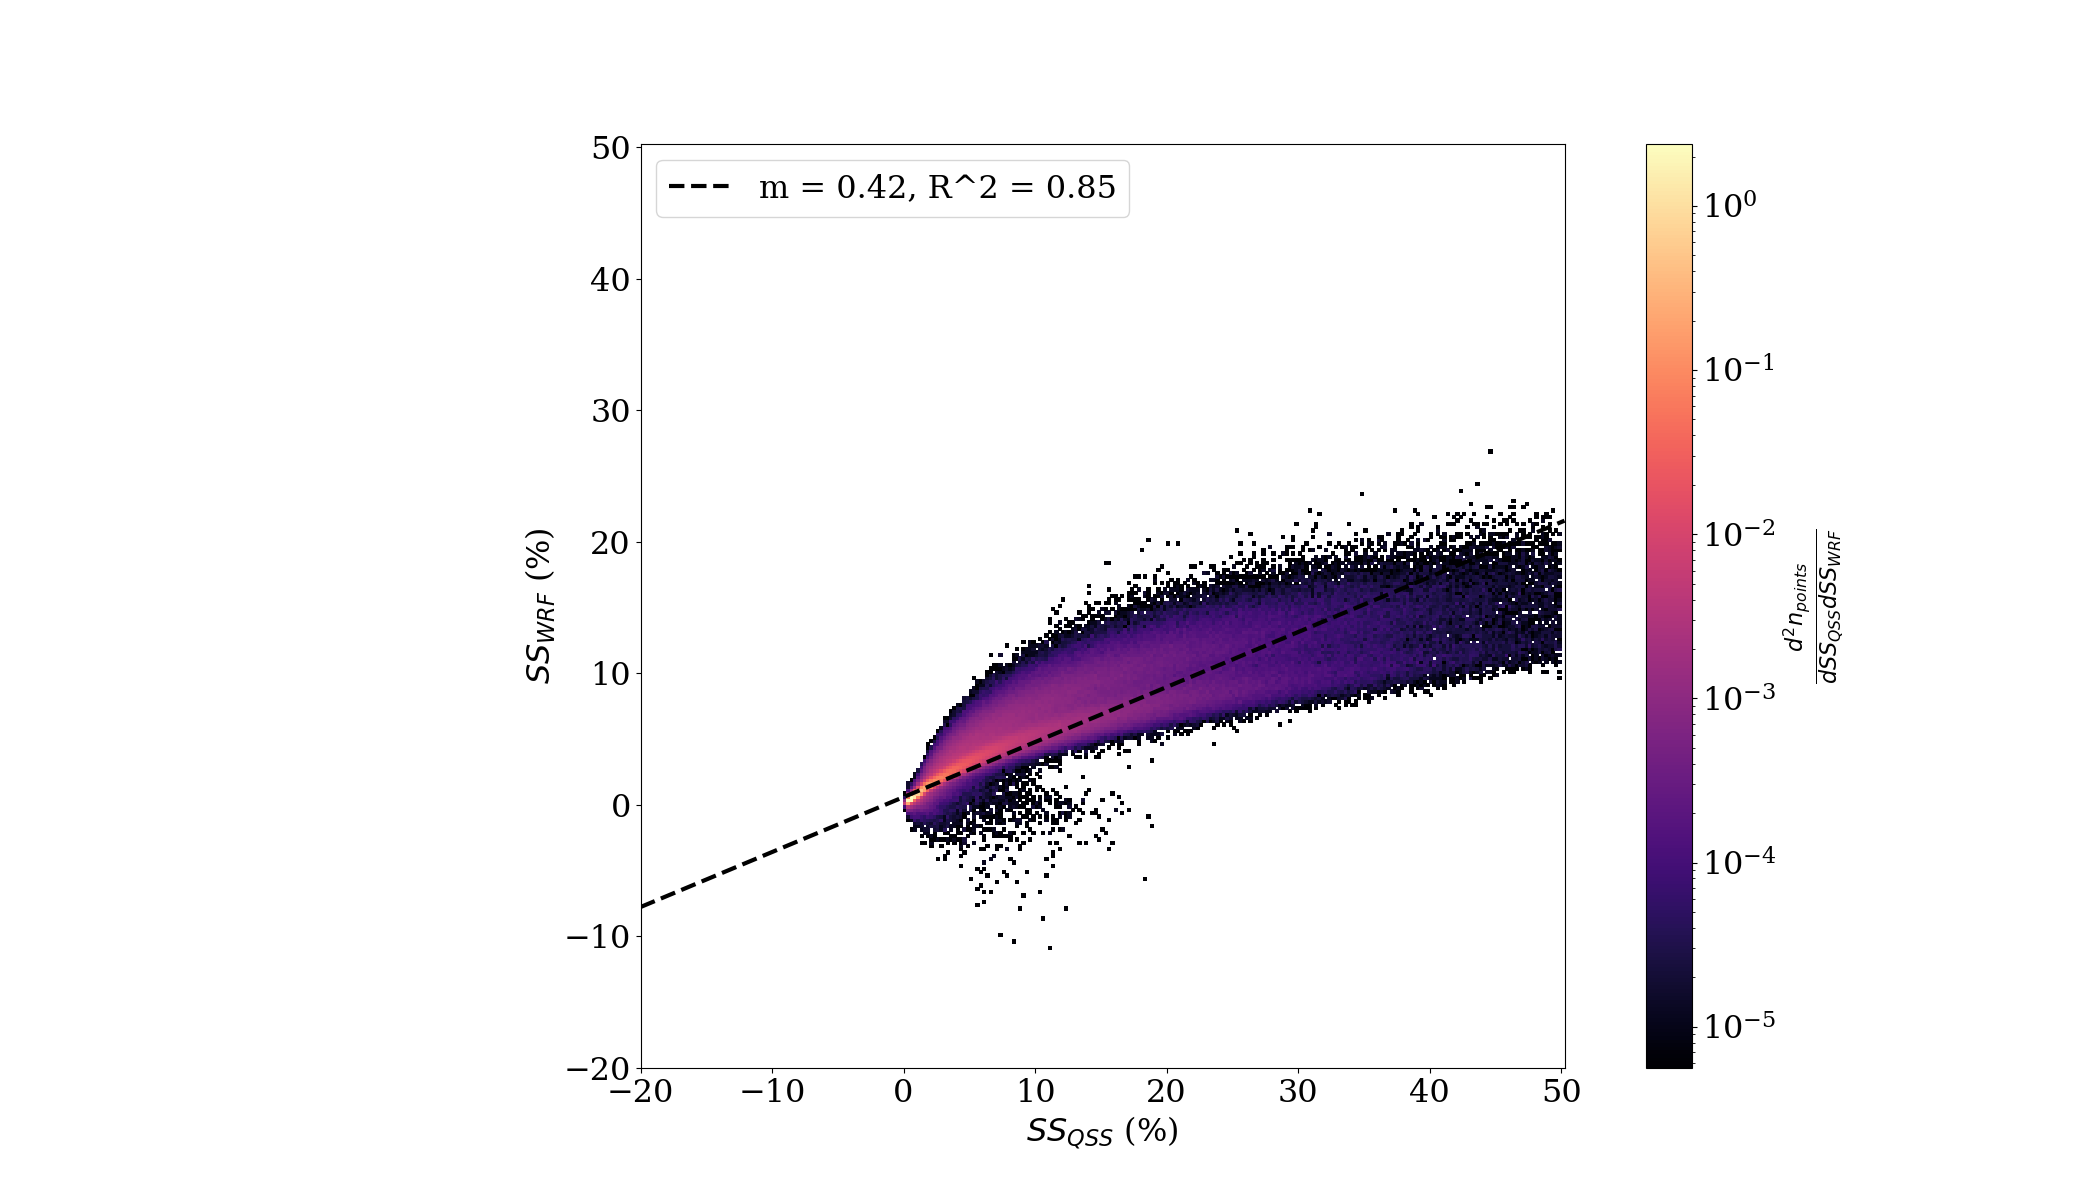
\includegraphics[width=\textwidth]{revmywrf/v5_FINAL_heatmap_ss_qss_vs_ss_wrf_Unpolluted_figure.png}
		\caption{Unpolluted case.}
		\label{wrfvsqssunpollv5}
	\end{subfigure}
	\begin{subfigure}{0.7\textwidth}
		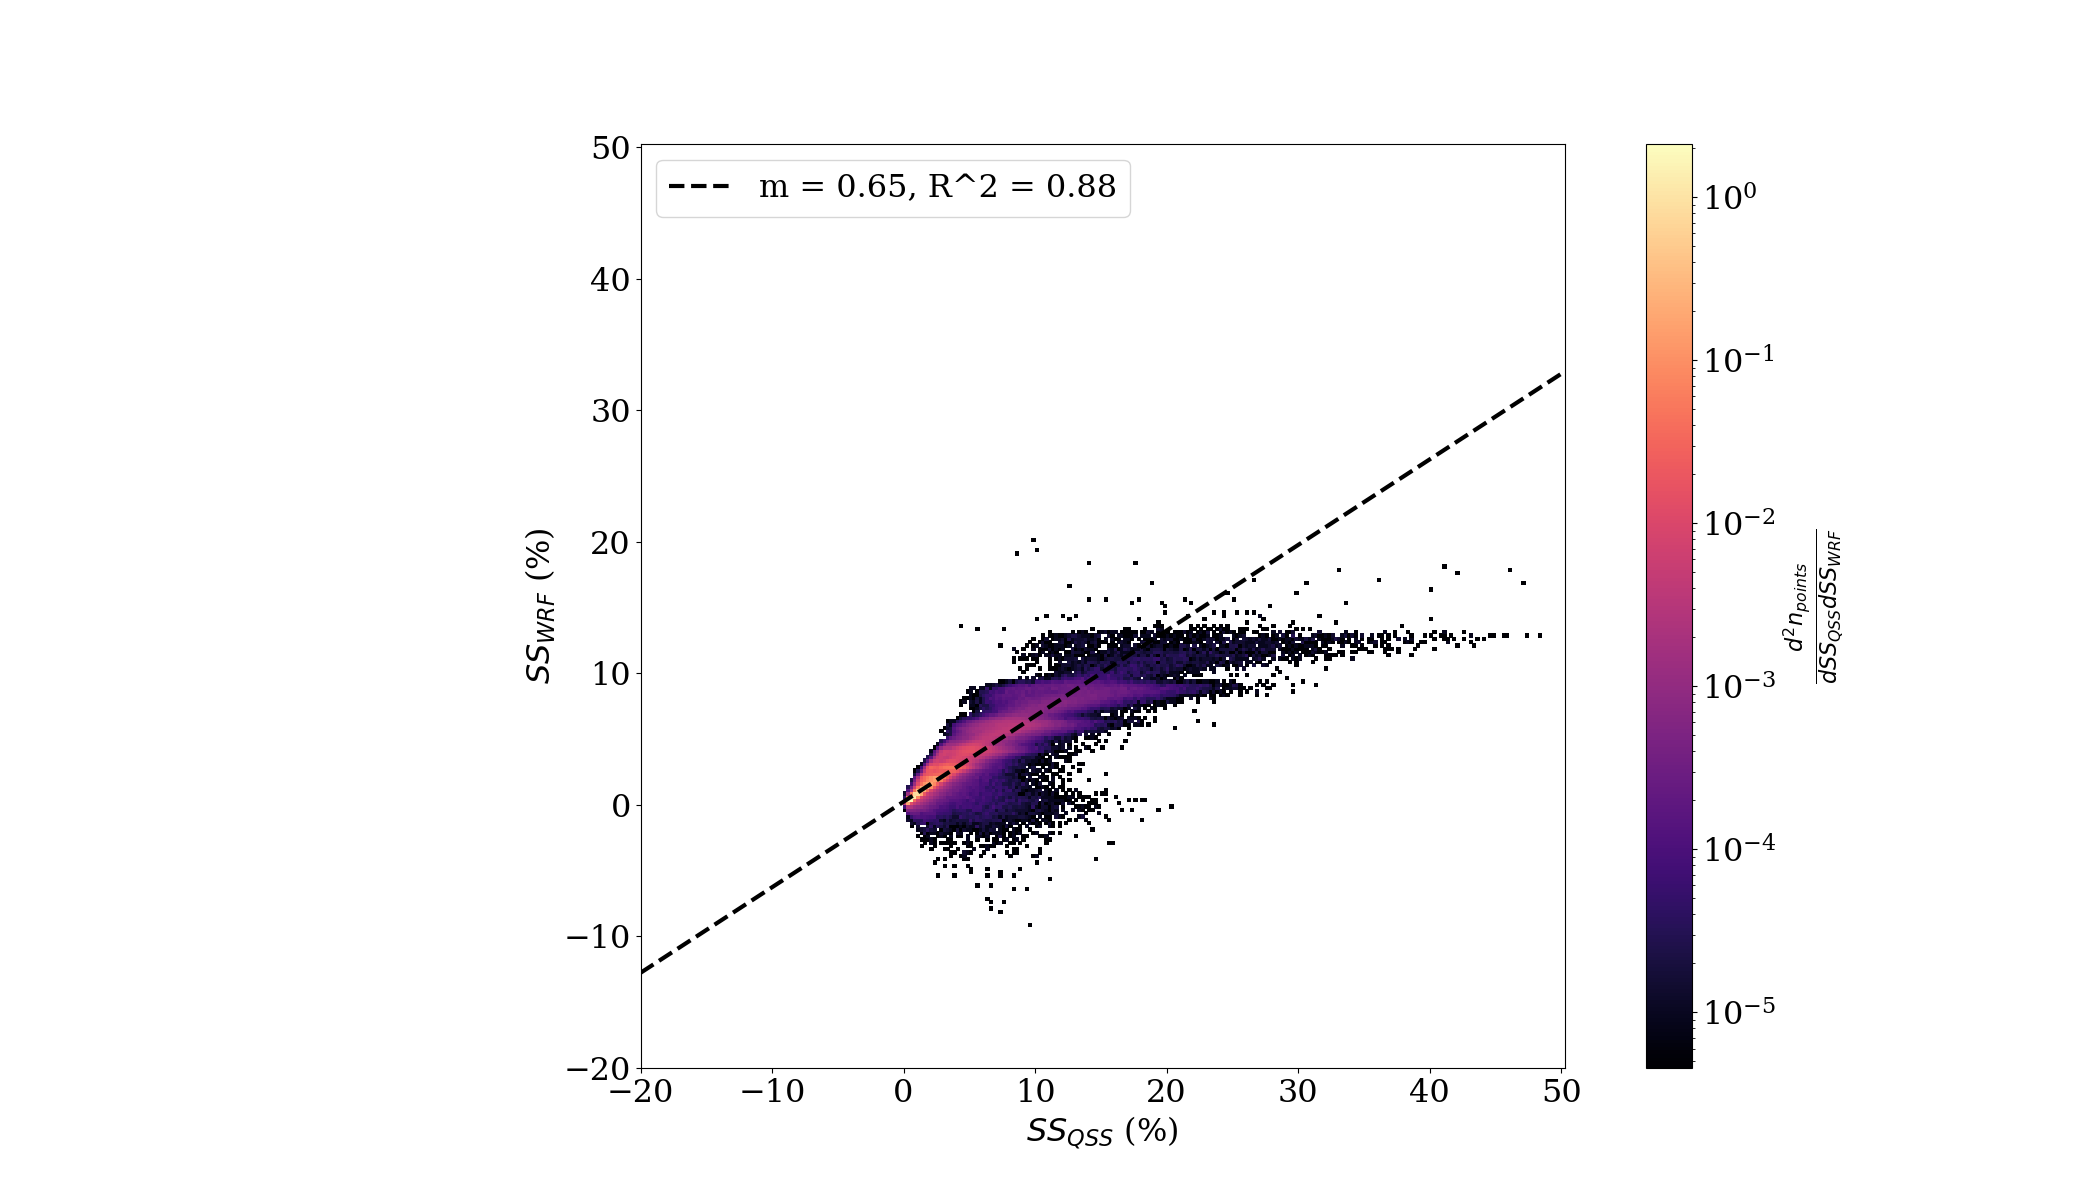
\includegraphics[width=\textwidth]{revmywrf/v5_FINAL_heatmap_ss_qss_vs_ss_wrf_Polluted_figure.png}
		\caption{Polluted case.}
		\label{wrfvsqsspollv5}
	\end{subfigure}
	\caption{Actual ($SS_{WRF}$) vs predicted ($SS_{QSS}$) supersaturation, without contributions from rain drops. Color indicates density of data points; note the scale is logarithmic.}
	\label{wrfvsqssv5}
\end{figure}

Finally, we note that we have excluded contributions to mean radius and number concentraiton from cloud droplets of diameter less than 5 $\mu$m, for consistency with our analysis of HALO data (see proceeding subsection). In the end this yields values for $SS_{QSS}$ which are indistinguishable to a reasonable number of significant figures.

\clearpage
\newpage

\subsection{HALO}

The HALO aircraft supported two instruments for measuring cloud droplet spectra: a cloud and aerosol spectrometer (CAS-DPOL) and a cloud droplet probe (one element of a cloud combination probe) (CCP-CDP) \cite{Braga2017}. We found that the CCP-CDP consistently reported unphysical bimodal size distributions, and therefore used only data from the CAS-DPOL for all calculations involving cloud droplets. Number concentrations from the CAS-DPOL were corrected using the $\xi$ factor derived in \cite{Weigel2016}.

The rain drop spectra came from data collected by greyscale cloud imaging probe (second element of the cloud combination probe) (CCP-CIP). The drop diameter detection ranges for CAS-DPOL and CCP-CIP were 0.89-50 $\mu$m and 25-2000 $\mu$m, respectively. Per guidance from the principal investigators for the CAS-DPOL, we only included data for droplets from size bins with a lower diameter bound greater than 3 $\mu$m in the analysis \cite{Jurkat2020}. Effectively (given size bins for this instrument), this meant that the lower bound on diameter for water drops was 5 $\mu$m. Because the CAS-DPOL and CCP-CIP have overlapping diameter detection ranges, we use concentrations for particles between 5 and 25 $\mu$m from CAS-DPOL and from 25 to 2000 $\mu$m from CCP-CIP. 

All measurements of environmental variables were taken from the Basic Halo Measurement and Sensor System (BAHAMAS). [TODO: details on time syncing]

[TODO: details on date selection]

We used the same Equation \ref{fullss} for $SS_{QSS}$ and for ventilation factors as described above.

\subsection{CAIPEEX}

Cloud droplet spectra for phase 1 of the CAIPEEX field campaign were measured by a CDP (detection range 2-1562.5 $\mu$m). We used the data from the following flight dates in 2009: 16, 21, 22 June; and 18, 23, 24, 25 August.

We used the same Equation \ref{fullss} for $SS_{QSS}$ and for ventilation factors as described above, and excluded data from cloud droplets of diameter less than 5 $\mu$m.

\begin{sidewaystable}[]
\centering
\begin{tabular}{@{}llll@{}}
\toprule
Symbol & Meaning & Value of constant & Notes \\ \midrule
$C_{ap}$ & Specific heat capacity at constant pressure, dry air & 1005 J/kg &  \\
$D$ & Molecular diffusion constant of water in dry air & 0.23e-4 m$^2$/s & We take as constant wrt T \\
$e_s$ & Saturation vapor pressure, water & - &  \\
$f(r)$ & Ventilation factor & - &  \\
$g$ & Gravitational acceleration on Earth & 9.8 m/s &  \\
$K$ & Coefficient of thermal conductivity in dry air & 2.4e-2 J/(m s K) & We take as constant wrt T \\
$LWC$ & Liquid water content & - &  \\
$L_v$ & Latent heat of vaporization, water & 2.501e6 J/kg & We take as constant wrt T \\
$N$ & Particle number concentration & - &  \\
$n_{points}$ & Point number density & - & Used for heatmap figures \\
$q_v$ & Water vapor mass mixing ratio & - & Equals $\frac{m_v}{m_{tot}}$ \\
$q_v^*$ & Saturation water vapor mass mixing ratio & - & Equals $\frac{m_v^*}{m_{tot}}$ \\
$r$ & Particle radius & - &  \\
$RH$ & Relative humidity & - & Equals $SS+1$ \\
$\rho_a$ & Mass density, dry air & - & Assuming ideal gas law \\
$\rho_w$ & Mass density, liquid water & 1000 kg/m$^3$ &  \\
$R_a$ & Ideal gas constant, dry air & 287.19 J/(kg K) &  \\
$R_v$ & Ideal gas constant, water & 460.52 J/(kg K) &  \\
$SS$ & Supersaturation & - & Equals $RH-1$ \\
$T$ & Temperature & - &  \\
$T_c$ & Temperature in degrees C & - & Equals $T – 273.15$ \\
$w$ & Vertical wind velocity & - &  \\
$z$ & Altitude & - &  \\ \bottomrule
\end{tabular}
\caption{Explanation of constants and variables used in the paper.}
\label{vartable}
\end{sidewaystable}

\clearpage
\newpage

\bibliography{refs}
\bibliographystyle{ieeetr}
\end{document}
